\newenvironment{spmatrix}[1]
{\def\mysubscript{#1}\mathop\bgroup\begin{pmatrix}}
	{\end{pmatrix}\egroup_{\textstyle\mathstrut\mysubscript}}
\newcommand*{\putunder}[2]{%
	{\mathop{#1}_{\textstyle #2}}%
}
\documentclass[onehalf,11pt]{beavtex}
\title{GPU-Based Fluid Structure Interaction using Immersed Boundary Methods}
\author{Christopher Minar}
\degree{Masters of Science}
\doctype{Masters Thesis}
\department{Mechanical Industrial and Manufacturing Engineering}
\depttype{School}
\depthead{Director}
\major{Mechanical Engineering}
\advisor{Kyle Niemeyer}
\submitdate{September 23, 2016}
\commencementyear{2016}
\abstract{Engineering applications often require fast, accurate solutions of fluid flow around freely moving bodies.
The massive parallelism enabled by GPU architecture enables high performance, offering a promising alternative to traditional solver acceleration via multicore CPUs.
However, fully harnessing GPU parallelism requires specialized algorithms and computing strategies.
This work modifies direct-forcing immersed boundary methods to model fluid-structure interaction and investigates its behavior on GPUs.
We performed verification of our solver using lid-driven cavity flow, impulsively started flow over a cylinder, flow over a forced oscillating cylinder and vorticity induced vibration.}
\acknowledgements{We gratefully acknowledge the support of NVIDIA Corporation with the donation of the Tesla K20 GPU used for this research.
We also thank the Barba Group for developing, maintaining, and distributing their cuIBM code.}

\usepackage{algorithm}
\usepackage{algorithmic}
\usepackage[textsize=footnotesize]{todonotes}%used for inline todo notes with \todo[]{}
\usepackage{latexsym,amsmath,amssymb} %math packages
\usepackage{tikz} %used for tikz graphics
\usepackage{standalone}  %used for tikz graphics
\usetikzlibrary{shapes}  %used for tikz graphics
\usepackage{amsmath} %used for matrix
\usepackage{graphicx} %needed for subfigure
\usepackage{float,caption,subcaption} %figure stuff
\graphicspath{{./figure/}} %figure path
\usepackage{siunitx}
\sisetup{group-separator={,},
	detect-all,
	binary-units,
	list-units = single,
	range-units = single,
	tophrase = --,
	per-mode = symbol-or-fraction,
	separate-uncertainty = true,
	list-final-separator = {, and }
}


\begin{document}
\maketitle

\mainmatter

\chapter{Introduction}
The 'Immersed boundary method' (IBM) is a broad term referring to a group of approaches used to simulate fluid flow over complex bodies.
The goal of IBMs is to represent a body surface withing resorting to a body fitted mesh.
These techniques are well-suited for simulating flow involving complex, moving bodies because they do not require re-meshing between time steps.
We have developed an IBM solver for operation on graphics processing units (GPUs) designed to handle incompressible fluid--structure interaction problems with rigid bodies.

Peskin~\cite{Peskin:1972gh} created the original IBM in the 1970s to model blood flow through arteries. 
He used the IBM to more easily represent the moving, elastic boundaries.
The original IBM adds a forcing term to the Navier--Stokes equations that represents the force a body would apply the fluid, if it were there.
This forcing term is modeled as a spring, $f=kx$, along with a Dirac-delta function to ensure the force only acts upon fluid nodes near the body.
Modeling the force as a spring worked well for Peskin's purpose but proved to have several shortcomings.
Firstly, solving for the forcing term is tedious, and the order of accuracy heavily depends on how it and the delta function are handled. \todo{site this}
Secondly, to apply the spring model to rigid bodies, a very large spring coefficient must be used which has the inadvertent effect of making the problem stiff. 

The IBM has since evolved to be applicable to a wide range of problems, as reviewed by Mittal and Iaccarino~\cite{Mittal:2005ii} and more recently Sotiropoulos and Yang~\cite{Sotiropoulos:2014gv}. 
The methods focused on in this work are all from a popular subgroup of IBM called direct forcing methods. 
Mohd-Yusof~\cite{MohdYusof:1997wh} and Fadlun et al.~\cite{Fadlun:2000fl} developed two early versions of direct forcing. 
In direct forcing, the velocities at the nodes nearest to the body are interpolated for using the body velocity, eliminating the need to solve for a forcing term while simultaneously enforcing the no-slip condition.
\todo[inline]{add segment about lee and lee}
However, using the direct forcing method with a moving body causes numerical oscillations~\cite{liao2010simulating}~\cite{Luo:2012gx}.
This effect is manageable for preset motion but with a freely moving body the solver will poorly predict body position, velocity, and forces. 
The numerical oscillations are caused by having different equations being used to solve for velocity in different regions of the domain. 
Luo et al.~\cite{Luo:2012gx} deals with the numerical oscillations by using a weighting function to transition between the two schemes, removing the discontinuity.

The goal of this project is to develop a GPU-based solver called cuIBM-FSI for CUda(CUDA is the language used to write for the GPU) Immersed Boundary Method Fluid Structure Interaction. 
The eventual purpose of cuIBM-FSI is to have a highly efficient solver to study and optimize wave energy converters. 
To those ends, this thesis will show that cuIBM-FSI capable of simulating 2D, incompressible flow over a freely moving body. 

Chapter \ref{chapter:Numerical Methods} will discuss the theory of several direct forcing methods and their applicability to freely moving bodies. 
Chapter \ref{chapter:Implementation} covers the discretization of various methods as well as the challenges, strategies and implementation of the GPU.
Chapter \ref{chapter:Validation} will show the validation and verification of different aspects of the solver using five different test cases; lid driven cavity, flow over an impulsively started cylinder, forced motion of a cylinder in static flow, forced motion of a cylinder in flow and vorticity induced vibrations (VIV). 
Chapter \ref{chapter:error} characterizes cuIBM-FSI in terms of order of accuracy and performance scaling. 
The final chapter will discuss the results, go over problems and recommend future work.

\chapter{Numerical Methods}\label{chapter:Numerical Methods}
cuIBM-FSI is comprised of three separate solvers. 
The first is modified from the work of Fadlun et al~\cite{Fadlun:2000fl}. 
Solvers two and three are both based off the work of Luo et al~\cite{Luo:2012gx}. 
For now, it will suffice to call these the modified Fadlun, external and embedded methods and leave their explanations for later. 


All of these methods, however, stem from the two-dimensional, incompressible form of the Navier--Stokes momentum and mass continuity equations:
\begin{align}
\frac{\partial \textbf{u}}{\partial t} + \nabla ( \textbf{uu} ) &= -\nabla p + \nu\nabla^{2}\textbf{u} \label{eq:NavierStokes} \\
\nabla \cdot \textbf{u} &= 0 \label{eq:Continuity} \;.
\end{align}
Here, $u$ is velocity, $p$ is pressure and $\nu$ is the constant kinematic viscosity.

\section{Navier--Stokes Fractional Step}\label{NM:NavierStokes}
All three methods use fractional step~\cite{Perot1993} to solve Equations \eqref{eq:NavierStokes} and \eqref{eq:Continuity}. 
The fractional step method breaks up the discretization of the Navier--Stokes equations. 
Specifically, each discretized time step is comprised of three sub steps.
In the first sub step, the momentum equations are solved without pressure to  calculate an intermediate velocity:
\begin{equation}\label{eq:Intermediate Velocity}
\hat{\textbf{u}} - \frac{\Delta t}{2}L(\hat{\textbf{u}}) = \textbf{u}^n + \Delta t(\textbf{RHS}^n) \;,
\end{equation}
where $\hat{\textbf{u}}$ is the intermediate velocity, $\Delta t$ is the time step, $L$ is the Laplacian operator and $\textbf{RHS}$ is the discretized advection and diffusion terms. 
The superscript $n$ represents the time step. 
In time, second-order Adams--Bashforth and Crank--Nicolson methods are used to discretize the advection and diffusion terms, respectively. 

In the second sub step, the continuity equation is imposed to approximate the pressure, $p$, resulting in the Poisson equation:
\begin{equation}\label{eq:Poisson}
\nabla^2p^{n+1} = - \frac{\nabla\hat{\textbf{u}}}{\Delta t} \;,
\end{equation}

Velocity is updated in the last sub step with:
\begin{equation}\label{eq:Projection}
\textbf{u}^{n+1} = \hat{\textbf{u}} - \Delta t\nabla p^{n+1} \;.
\end{equation}

\section{Node Identification}
To facilitate the discussion of IBMs the nomenclature with regards to point identification will be explained here. 
The nomenclature is mostly adopted from the work of Luo et al.\cite{Luo:2012gx}
There are four types of nodes. 
Not all of them are used in each method, and the methods treat nodes differently. 
Nodes immediately outside the body are hybrid nodes. 
In all three methods, the hybrid nodes are interpolated for using the body and second nearest node. 
Nodes immediately inside the body are ghost nodes. 
The Fadlun(and modified Fadlun) method doesn't use these but the external and embedded methods both try to set these values in a way that enforces the body, more on this in section~\ref{Sec:Field Extrapolation}. \todo[inline]{cite mittal?}
Everything outside of the body that ins't a hybrid node is a fluid node. 
Fluid nodes are solved by the unmodified Navier--Stokes equations. 
Everything else (all nodes inside the body that are not ghost nodes) are solid nodes. 
The treatment of solid nodes doesn't effect the solution. 
It does effect the computational time. 
The Poisson equation tends to solve the fastest when a standard five point stencil is used. 
When the solid nodes use a five point stencil an arbitrary flow field will develop inside the body. \todo{this section is sloppy and could use some tinkering}
Figure~\ref{fig:node id} demonstrates. 

\begin{figure}[!htb]
	\centering
	\includestandalone[width=0.5\linewidth]{node_id}
	\caption{Node identification near the body}
	\label{fig:node id}
\end{figure}

\section{Fadlun}
In Peskin's\cite{Peskin:1972gh} original IBM(Peskin has developed many iterations of the IBM) a forcing term $f$ in Equation \eqref{eq:NavierStokes} is solved for at the hybrid nodes in a way that enforces no-slip. 
In the direct forcing methods developed by Fadlun\cite{Fadlun:2000fl} and Yusof\cite{MohdYusof:1997wh} the Navier--Stokes equation isn't solved at the hybrid nodes. 
Instead, the velocity at the hybrid node is approximated by linearly interpolating between the second closest node and the body surface as seen in Figure~\ref{fig:2}. 
\begin{figure}[!htb]
	\centering
	\includestandalone[width=0.5\linewidth]{basic_interp_figure}
	\caption{A simplified diagram of linear interpolation for velocity values at a hybrid node}
	\label{fig:2}
\end{figure}
At this point a clever observer might notice a complication induced by the fractional step method. 
Which is correct, to enforce no slip to the intermediate velocity in the first sub step, or to velocity during the third sub step? 
Fadlun found that when no-slip is applied during the intermediate time step, the error introduced in the velocity correction step was always negligibly small compared to the velocity. 
\todo[inline]{when is this approximation not viable?}
$\textbf{RHS}$ and $1-\frac{\Delta t}{2}L$ from Equation \eqref{eq:Intermediate Velocity} can be setup as if they was no body, then modified at the hybrid nodes to enforce no slip with the linear interpolation. 
The discretization of this is shown in appendix \ref{Fadlun Linear Interpolation}. 
The Poisson Equation \ref{eq:Poisson} and projection step \ref{eq:Projection} are left unmodified in the work of Fadlun et al. 

\section{Modified Fadlun} 
In the impulsively started cylinder simulation, section \ref{sec:cylinder}, the Fadlun method proved mediocre at predicting force in the transient section (while the boundary layer was developing). 
This happens because the Poisson equation is not modified to account for the presence of a body causing the continuity equation will not be satisfied. 
There are many proposed and tested solutions to this issue. 
Depending on the type of simulation this can create significant creation or destruction of mass at the body, leading to poor solver accuracy.
Kim et al~\cite{kim2001immersed}. added mass source or sink terms to the continuity equations at cells cut by the body surface. 
Mittal et al\cite{mittal2008versatile}. imposes no-slip by extrapolating velocity data outside the body to ghost nodes. 
Luo et al\cite{Luo:2012gx}. also extrapolates inwards in addition to enforcing an approximate pressure boundary condition. 
cuIBM-FSI's modified Fadlun method uses a cut cell approach to fix the mass continuity issue. 
This is explained in more detail in section~\ref{sec:modified fadlun}.

\section{Luo}

Direct forcing methods suffer from numerical oscillation when the immersed body is moving~\cite{Sotiropoulos:2014gv}~\cite{Mittal:2005ii}~\cite{liao2010simulating}.
As the body moves, background nodes change how they calculate values. 
For example Figure~\ref{fig:Temporal Discontinuity} depicts a bulk fluid $u$ velocity node at time step $t^n$ become a hybrid node at time step $t^{n+1}$.
As the node transitions the intermediate velocity will change from being calculated by Navier--Stokes (Equation ~\eqref{eq:Intermediate Velocity}) to an interpolation (Equation~\eqref{eq:ID intermediate velocity interpolation} or \eqref{eq:Interpolation}). 
Both equations are correct representations for the intermediate velocity but they have different errors associated with them which causes the calculated velocity to be slightly different. 
This discontinuous change in velocity is responsible for the numerical oscillations. 
Note that this effect happens whenever any node transitions, not just the intermediate $u$ velocity nodes.

\begin{figure}[!htb]
    \centering
    \includestandalone[width=0.5\linewidth]{figure/node_transition_figure}
    \caption{A diagram illustrating the immersed body's interaction with the background grid that causes numerical oscillations.}
    \label{fig:Temporal Discontinuity}
\end{figure}

In the method proposed by Luo et al.~\cite{Luo:2012gx}, hybrid node values are calculated via both Navier--Stokes and interpolation.
The final value at the hybrid node is a weighted combination of both solutions. 
The weighting is designed smooth the transition between solutions. 
When the hybrid node is close to the body, it will be dominated by the interpolated solution, while a the hybrid node far from the body will be dominated by the Navier--Stokes solution. 
This process is elaborated on in section \ref{Sec:Weighting}. 
To get a valid result at the hybrid nodes using the Navier--Stokes equations the field values (velocity and pressure) must be extrapolated across the body using appropriate boundary conditions. 
This process is elaborated on in section \ref{Sec:Field Extrapolation}. 


\subsection{Field extrapolation to ghost nodes}
\label{Sec:Field Extrapolation}

Navier--Stokes can be used to calculate values at the hybrid nodes if the ghost nodes are modified to correctly represent the presence of the body. 
If the slope of velocity between the hybrid node and the body is assumed to be linear then the slope can be extrapolated inwards to the ghost node. 
A simple example of this can be seen in Figure~\ref{Fig: Simple Interpolation}. 
The ghost node is set such that the velocity is zero via linear interpolation between the ghost and hybrid nodes. 
When Navier--Stokes is then solved, the fluid velocity at the body surface will be calculated as the velocity of the body, mimicking the no slip boundary condition. 
\begin{figure}[!htb]
	\centering
	\includestandalone[width=0.5\linewidth]{basic_extrapolation}
	\caption{A simple 1D, linear extrapolation example}
	\label{Fig: Simple Interpolation}
\end{figure}
In the actual Luo et al~\cite{Luo:2012gx}. method, field values are extrapolated across the body using 2D bilinear interpolation.
Unlike Luo et al., cuIBM-FSI uses a staggered grid, causing the extrapolation process to have three variations; one for pressure and ones for $u$ and $v$ velocity nodes. 
Values are first interpolated for at an image point outside the body using the surrounding field values and the boundary condition. 
The 2D bilinear interpolation approximates the field between four nodes surrounding the image point with Equation~\eqref{eq:Interpolation}. 
Each node surrounding the image point is used to set up a system of four equations to solve for the coefficients of~\eqref{eq:Interpolation}, which can then be used to solve for the field values. 
Some of the interpolation nodes will be moved to account for the presence of the body.
In Figure~\ref{fig:Ghost node extrapolation} the bottom left corner of each interpolation region is moved to the body intercept.
\begin{figure}[htb]
	\centering
	\includestandalone[width=0.5\linewidth]{GN_interp_figure}
	\caption{A detailed schematic $u$ velocity extrapolation to ghost nodes.}
	\label{fig:Ghost node extrapolation}
\end{figure}

The ghost nodes, indicated by solid squares, are projected onto the surface to find the body intercept, indicated by the thick open circle. 
Body nodes used to track the body's position are not the same as the body intercept and the two are typically not coincident. 
If the body has curvature, the body intercept will not fall exactly on the body due to the discrete representation of the body. 
The line drawn between the body intercept and ghost node will be perpendicular to the tangent line at the body intercept, i.e. the ghost node is projected along the surface normal. 
That line is then mirrored over the surface to find the image point, indicated by the solid triangle. 

The rules to determine which values are used to interpolate for the image point are as follows:
If one of the four interpolation nodes is inside the body, as seen in the extrapolation for GN 1 in Figure~\ref{fig:Ghost node extrapolation}, then that node is moved to the body intercept and the boundary condition is used. 
It is possible for multiple corners to be inside the body. 
Any corner inside the body will always be a ghost node and have its own, corresponding body intercept. 
All corners inside the body are moved to their corresponding BI such that there are always four corners in separate locations to use for the interpolation. 
If none of the four field values are inside the body as seen in the extrapolation for GN 2 then the node closest to the body intercept is moved to the body intercept.
To satisfy the no slip condition at the body, a Dirichlet boundary condition equal to the body velocity is used when extrapolating for velocity ghost nodes. 
The pressure boundary condition is approximated by forcing the slope of pressure normal to the body surface, $\frac{dp}{dn}$, as constant using the Neumann Equation~\eqref{eq:Neumann}. 
Using the relocated corners, a system of equations is set up to solve for the coefficients in Equation~\eqref{eq:Interpolation}.
Pressure nodes on the body use Equation~\eqref{eq:Neumann Node} in the system, which is simply the derivative of Equation~\eqref{eq:Interpolation}. 
\begin{align}
\phi (x,y) = a_0 + a_1 x + a_2y + a_3 x y \label{eq:Interpolation} \\
\phi (x,y) = a_1 + a_2 + a_3 (x+y) \label{eq:Neumann Node} \\
\left. \frac{\partial p}{\partial \textbf{n}}\right|_{BI} = \left. -\rho \frac{D\textbf{u}}{Dt}\cdot \textbf{n}\right|_{BI}
\label{eq:Neumann}\;.
\end{align}
$\phi$ is the variable being interpolated ($u$, $v$, or pressure); $a_0$, $a_1$, $a_2$ and $a_3$ are coefficients, and $x$ and $y$ give the node location.
$\rho$ is the density, $D\textbf{u}\left/Dt\right.$ is the material derivative, and $\textbf{n}$ is the unit vector normal to the body.
Solving this system on the GPU requires direct inversions of the $4 \times 4$ matrices.
This process is elaborated on in \ref{system of euqations}. 
Once the $a$ coefficients have been found, the field value at the image point can be calculated with equation~\eqref{eq:Interpolation} and extrapolated across the surface using equation~\eqref{eq:Velocity Interpolation} for velocity or ~\eqref{eq:Pressure Interpolation} for pressure. 
$\Delta l$ is the distance from ghost node to image point.
\begin{align}
\textbf{u}_{GN} &= 2\textbf{u}_{BI} - \textbf{u}_{IP} \label{eq:Velocity Interpolation} \\
p_{GN} &= p_{ip} - \Delta l \left. \frac{\partial p}{\partial \textbf{n}}\right|_{BI} \;, \label{eq:Pressure Interpolation}
\end{align}

\subsection{Interpolation to hybrid nodes}
\label{Sec:Interpolation}

Interpolating for the field value at the hybrid node is largely the same as interpolating for the ghost nodes' image point described previously. 
The body intercept is once again found by projecting the hybrid node along the surface normal. 
The image point is not used in the same way as the ghost node image point is. 
If a given body intercept is located at $(x_{BI},y_{BI})$ and its hybrid node is located at $(x_{BI}+\Delta x,y_{BI}+\Delta y)$ the corresponding image point is located at $(x_{BI}+2\Delta x,y_{BI}+2\Delta y)$ as shown in Figure~\ref{fig:Interpolate}. 
In hybrid node case, an image points only purpose is locating the four interpolation nodes, one of which will always be the corresponding hybrid node. 
The interpolation node coincident with the hybrid node is moved to the body intercept and the appropriate boundary condition for velocity or pressure is applied.
Once equation~\eqref{eq:Interpolation} is solved, the hybrid node is interpolated for.
Details on this process can be found in \ref{a: interpolation to hybrid nodes}. 
\todo[inline]{deal with this}
\begin{figure}[!htb]
	\centering
	\includestandalone[width=0.5\linewidth]{HN_interp_figure}
	\caption{A detailed schematic of the hybrid node interpolation.}
	\label{fig:Interpolate}
\end{figure}

\subsection{Weighting}
\label{Sec:Weighting}

Instead of the Dirac-delta style transition at the body of traditional direct forcing methods, Luo et al.~\cite{Luo:2012gx} introduced a smooth transition between solution regimes.
Its purpose is to dampen the numerical oscillations that results from the discontinuous switch. 
The scalar $\alpha$ is introduced to the solutions for intermediate velocity and the pressure:
\begin{equation}\label{eq:Weight}
\theta = \left(1-\alpha \right)\theta_{Navier-Stokes} + \alpha \theta_{Interpolated} \;,
\end{equation}
where $\theta$ represents either intermediate velocity or pressure.
Transitioning between the Navier--Stokes and interpolated solutions should meet three criteria:
\begin{enumerate}
	\item Hybrid nodes farther from the body should favor the Navier-Stokes solution ($\alpha \rightarrow 0$ as distance $\uparrow$).
	\item Hybrid nodes closer to the body should favor the interpolated solution ($\alpha \rightarrow 1$ as distance $ \rightarrow 0$).
	\item The weighting function should be smooth and continuous as the hybrid node moves away from the body.
\end{enumerate}
To solve for $\alpha$, it is assumed that each hybrid node has at most two neighboring ghost nodes (this will not be true for sharp corners):
\begin{equation}
\alpha = \sqrt{\left(\frac{\Delta_1}{\Delta x}\right)^2 + \left(\frac{\Delta_2}{\Delta y}\right)^2} \;.
\label{eq:Alpha}
\end{equation}
where $\Delta_1$ and $\Delta_2$ correlate to GN$_1$ and GN$_2$, respectively, and $\Delta x$ and $\Delta y$ are the grid spacing in the $x$ and $y$ directions, respectively. 
As described in Luo et al. and shown in Figure~\ref{fig:Weight}, $\Delta_1$ and $\Delta_2$ are the closest distances between the body and the $x$ and $y$ ghost nodes, respectively. 
If the hybrid node only has one neighbor, then $\Delta=0$ for the other direction. 
\begin{figure}[htb]
	\centering
	\includestandalone[width=0.5\textwidth]{alpha_figure}
	\caption{Schematic of the calculation of $\alpha$ for u velocity nodes.}
	\label{fig:Weight}
\end{figure}

\chapter{Implementaiton and Discretization}\label{chapter:Implementation}

This chapter will detail the discretization of the immersed boundary method and implementation on the GPU. 
\todo[inline]{need more here, perhaps a summary of each section?}

\section{Sparse Matricies}
When using a dense matrix, every possible spot in the matrix has a physical location in memory. 
The matrix that represents the coefficients for intermediate velocity and pressure are comprised of mostly zeros. 
It is inefficient to store the entirety a so called sparse matrix. 
cuIBM-FSI stores sparse matrices in the COO format. 
A COO matrix stores each entry as three values, row, column and value. 
CUSP represents each COO matrix as three separate arrays. 
On a CPU as each node is stepped through its values can be added to the next location in the COO arrays. 
If a GPU were to attempt this, a race condition would occur. 
To prevent the race condition each node must have a predetermined location in the array. 
Nodes at the corners, sides and center of the domain have three, four and five matrix entries, respectively. 
This is determined by how many neighbors each node depends on. 
Each GPU thread calculates the total entries before it and starts placing its nodes appropriately. 
The nodes are counted from left to right, top to bottom. 
In the kernel that generates the COO matrix, each node will be handled by a single thread. 
The thread knows the first array location and the number of entries it should be adding, which it then does at it sees fit.

\section{GPU implementation strategy}
\label{GPU implementation strategy}
\todo[inline]{make a picture to demonstrate why divergence is acceptable}
cuIBM-FSI is developed for full GPU operation to improve performance relative to CPU-based algorithms. 
To this end, several overarching strategies have been implemented. 
First, all calculations are performed on the GPU, and all data is stored on the GPU.
Typically, efforts are taken to avoid thread divergence when writing code for a GPU. 
We found it favorable to write kernels with occasionally poor thread-parallel performance, i.e., kernels with significant divergence, rather than copying data to the host to do calculations to reduce divergence. 
Increasing the parallel performance of kernels has little effect on the overall solver performance because solving the Poisson equation typically takes more than \SI{90}{\percent} of the total computational time. 
In our experiences, transferring data back and forth took significantly more time than would be saved by running some operations on a CPU. 
This is particularly relevant when moving from a stationary body to a moving body.
When simulating a stationary body, several calculations only need to be performed once, such as the left side matrices, node identification and preconditioners.
When simulating a moving body, these values need to be recalculated every time step, causing a total computational cost for each nearly as high as the Poisson equation solve (typically the most expensive step). 
This relates to the second strategy: evaluate algorithm performance compared to the Poisson equation. 

The third strategy comes from Layton et al.~\cite{layton2011cuibm}.
When using the Cusp library to perform the multigrid method, creating the preconditioner can take as much time as solving the Poisson equation.
In a moving-body simulation, the preconditioner is normally recalculated each time step, but Layton et al.~\cite{layton2011cuibm} found it possible to skip some time steps without loss of fidelity.
Here, we recalculate the preconditioner only if solution of the previous time step required more than 100 iterations. 
The external method does not need the preconditioner to be remade, even when its moving, because each node always depends on the same things regardless of the position of the body. 


\section{Grid Staggering}
\label{Grid Staggering}

A collocated grid stores all variable information at the center of each cell.
When discretized on a collocated grid, Navier--Stokes will yield an odd-even decoupling of pressure an velocity resulting in a checkerboard pattern unless special steps are taken to prevent it. 
\todo[inline]{findsource for this info}
Using a staggered grid is a relatively straightforward way to avoid odd-even decoupling.
A staggered grid stores scalar values(pressure, temperature, density etc.) at the cell center and velocities at the cell face. 
Staggered grids also have the advantage of not requiring a pressure boundary condition.
cuIBM-FSI is staggered in the positive x and y directions. 
That is, if the cell center is cell denoted as i as shown in Figure~\ref{fig:stagger}, the top and right faces are also denoted as i and the bottom and left faces are i-nx and i-1. 
It is worth noting that Luo et al.\cite{Luo:2012gx} uses a collocated grid.
Due to the sensitivity of immersed boundary methods near the body, this may cause some difference.
There is no theoretical reason why the numerical suppression method should not work on a staggered grid.
\begin{figure}[!htb]
	\centering
	\includestandalone[width=0.5\textwidth]{grid_stagger}
	\caption{Grid staggering: The velocities are staggered in the positive x and y directions.}
	\label{fig:stagger}
\end{figure}

\section{Node Identification}
Nodes are identified using a ray tracing algorithm described in the book Computational Geometry in C by Joesph O'Rourke\cite{o1998computational}.
The implementation is based of the CPU implementation from the original cuIBM. \todo{get citation for cuIBM}
One thread is generated for each node, be it u, v or pressure and performs the following actions to find rays in the x direction.
First the Lagrangian body nodes are looped through to make segments with their nearest neighbors.
If to top of this segment is above the node and the bottom of the segment is below the node then the x location of the body at the height of the node is found(open circle in Figure~\ref{fig:node id 1}).
The node is then tested for proximity to the body in the x direction. 
To determine what the node is, five x-coordinates are used; $x_{i-1}$, $x_{i}$, $x_{i+1}$, $x_{BI}$ and $x_{body center}$. 
Using Figure \ref{fig:node id 1} for example, the BI will text as being greater than the body center, greater than $x_{i-1}$ and less than $x_{i}$ which makes $u_{i,j}$ a hybrid node. 

It is possible for a hybrid or ghost node to be unable to find the body when searching in the x direction, i.e. if the node is above the highest body node.
After the algorithm looks for intersections in the x direction it searches in the y direction.
In the case where a node is able to find the body in both the x and y directions, the x direction is always chosen. 
The v velocity and pressure nodes are found in the same way as described above, but use different coordinates.

After all the points have been tagged, the solid nodes are set to an arbitrary value so they can be easily found later.
This step is not critical for Navier--Stokes but is needed for the force calculation, which disregards everything inside the body, and can be convenient when visualizing the solution.
\begin{figure}
	\centering
	\includestandalone[width=0.5\textwidth]{node_id_1}
	\caption{To find the hybrid and ghost nodes the position of the body must be translated from the Lagrangian body nodes to the Eulerian grid.}
	\label{fig:node id 1}
\end{figure}

\section{Force Calculation}
\label{Force Calculation}

The drag and lift on the body are calculated using the control volume approach detailed in Lai and Peskin\cite{lai2000immersed}.
The implementation of this approach is largely the same as the original cuIBM. 
Lai and Peskin give Equation~\eqref{eq:force calculation} to calculate the drag force. 
\begin{equation}\label{eq:force calculation}
F_D=-\int_{\partial \Omega_0} \rho u_i\textbf{u}\cdot \textbf{n}ds- \int_{\partial \Omega_0}pn_ids+\int_{\partial \Omega_0}\mu \left(\frac{\partial u_i}{\partial x_j}+\frac{\partial u_j}{\partial x_i}\right)n_jds-\frac{\partial}{\partial t}\int_{\Omega_0}\rho u_i d\textbf{x}
\end{equation}
$\Omega_0$ is any square sub-domain place around the body. 
Once discretized, simplified, non-dimensionalized the terms can be rearranged into 3 groups, FxX, FxY and FxU. 
The first term represents the forces in the x direction from the left and right of the control volume and is formed from the second and third integral in \eqref{eq:force calculation}. 
FxY is the forces in the x direction from the top and bottom of the control volume.
It comes from the first and third integral. 
The fourth integral becomes FxU, the x force from the unsteady term and includes everything inside of the control volume. 
These terms are partialy discretized in equations \eqref{eq:force calculation 2}, \eqref{eq:force calculation 3} and \eqref{eq:force calculation 4}. 
\begin{align}
FxX &=-\sum_{\Omega_y}\left((p_e-p_w)+(u_e^2-u_w^2)-\nu\left(\left.\frac{du}{dx}\right|_e-\left.\frac{dv}{dx}\right|_w\right)\right)dy\label{eq:force calculation 2}\\
FxY &=-\sum_{\Omega_x}\left(0.5(u_nv_n-u_sv_s)-0.25\nu \left(\left.\frac{du}{dy}\right|_n+\left.\frac{dv}{dx}\right|_n-\left.\frac{du}{dy}\right|_s-\left.\frac{dv}{dx}\right|_s\right)\right)\label{eq:force calculation 3}\\
FxU &=\frac{u_i^{n+1}-u_i^{n}}{dt}0.5dydx\;\label{eq:force calculation 4}
\end{align}
The subscripts n,e,s,w represent the north, east, south and west faces of the sqaure domain $\Omega_0$.
In practice, varying the size of $\Omega_0$ from L=4 to L=10 was not found to have a significant effect on the force or computation time.
It was also found that the body didn't have to be at the center of the domain.
Given this, the control volume is generally kept in the same location as the body moves around inside it.
We typically used a square with sides L=10 for a body of size D=1 that moves about 1D away from center.

Depending on how the ghost and solid nodes are handled Equation \eqref{eq:force calculation} can predict force very poorly.
To circumvent this effect over multiple solvers all nodes inside the body are excluded from the unsteady term.

\section{Linear Algebra}
\label{Preconditioning and Linear Algebra Solvers}
CUSP(cuda sparse) is the linear algebra library used by cuIBM-FSI. 
CUSP can handle many different types of sparse data structures and has several different solvers built in. 
cuIBM-FSI uses a bi-conjugate gradient stabilized(BiCGSTAB) method for both the intermediate velocity and Poisson equation. 
Preconditioners are used to improve performance. 
A diagonal preconditioner is used for the intermediate velocity and a smoothed aggregation for the pressure step. 
Smoothed aggregation is a type of multi-grid approach to linear algebra that can drastically speed it up. 
In a multi-grid method, several iterations of BiCGSTAB(or any convergence method) are done on the full grid, then the solution is transfered to a coarser grid. 
This process is repeated until the grid is very coarse and then the solution is rebuilt on finer and finer grids until a solution has been obtained for the full grid. 
Getting an approximation to the matrix's inverse using the coarser grids saves computational time. 
\section{Navier--Stokes}
\label{ID:Navier Stokes}

The 2D incompressible Navier--Stokes equation forms the backbone of the immersed boundary method. 
To solve Navier--Stokes, the fractional step method is used. 
In the first step, Equation~\eqref{eq:Incompressible NavierStokes} drops the pressure term and is discretized to get an intermediate velocity. 
\begin{equation}
\frac{\partial \textbf{u}}{\partial t} + \nabla ( \textbf{uu} ) = -\nabla p + \nu\nabla^{2}\textbf{u} \label{eq:Incompressible NavierStokes}
\end{equation}
In the second sub step, Equation~\eqref{eq:Poisson} is solved for pressure. 
In the third sub step, the final velocity is updated. 
This section goes over the discretization details of using fractional step for normal Navier--Stokes. 
Sections~\ref{sec:ID fadlun}, \ref{sec:ID external} and \ref{sec:ID embedded} cover the modifications required for the presence of an immersed boundary with the modified Fadlun, external and embedded methods. 

\subsection{Intermediate Velocity}
\label{sec:ID NS intermediate velocity}

The advection term, $\nabla (\textbf{uu})$, is discretized in time using explicit, second-order Adams-Bashforth. 
Diffusion, $\nu \nabla^2 \textbf{u}$, is discretized using Crank-Nicolson. 
The result is an expanded form of Equation\eqref{eq:Intermediate Velocity}, Equation~\eqref{eq:Expanded Intermediate Velocity}. 
\begin{equation}
\label{eq:Expanded Intermediate Velocity}
\hat{\textbf{u}} - \frac{\Delta t}{2}L(\hat{\textbf{u}}) = \textbf{u}^n + \Delta t\left(0.5L(\textbf{u}^n) - 1.5N(\textbf{u}^n) + 0.5N(\textbf{u}^{n-1}) + BC\right)
\end{equation}
Where $N$ is the advection operator, $L$ is the diffusion Laplacian operator and $BC$ is the boundary condition term which is the leftovers from applying the Laplacian to $\hat{\textbf{u}}$. 
Each term, N, L, BC, LHS, is described in its own section below. 

\subsubsection{Advection}
\label{sed:ID NS Advection}
The advection term, $\nabla (\textbf{uu})$, expands to become Equations~\eqref{eq: Advection 1} and~\eqref{eq: Advection 2} which are in the x-momentum and y-momentum equations, respectively. 
Due to the staggered grid, the discretization of Equations~\eqref{eq: Advection 1} and~\eqref{eq: Advection 2} are slightly different but for brevity only the discretization of x-momentum will be shown. 
Note that $u$ and $v$ represent scalar velocities but $\textbf{u}$ is a vector. 
\begin{align}
&u\frac{\partial u}{\partial x} + v\frac{\partial u}{\partial y} \label{eq: Advection 1} \\ 
&u\frac{\partial v}{\partial x} + v\frac{\partial v}{\partial y} \; \label{eq: Advection 2}
\end{align}
Discretizing \eqref{eq: Advection 1} on a uniform grid using second order central differencing results in Equation~\eqref{eq: discretized uniform advection}. 
Figure~\ref{fig:discretized uniform advection}a shows a section of uniform grid for reference with Equation~\eqref{eq: discretized uniform advection}. 
A non-uniform grid requires a more involved discretization, shown in \eqref{eq: discretized nonuniform advection} and \eqref{eq:bili 3}. 
If $\Delta x_{i+1}$ does not equal $\Delta x$ then $\frac{\partial u}{\partial x}$ must be calculated at the cell centers, indicated by the open circles marked $1$ and $2$ in Figure~\ref{fig:discretized uniform advection}b, then interpolated to $u_{i,j}$. 

\begin{align}
u_{i,j}\frac{u_{i+1,j} - u_{i-1,j}}{2dx} &+ \frac{v_{i,j} + v_{i+1,j} + v_{i,j-1} + v_{i+1,j-1}}{4}\frac{u_{i,j+1} - u_{i,j-1}}{2dy} \label{eq: discretized uniform advection}\\
\left.\frac{du}{dx}\right|_i&=\left.\frac{du}{dx}\right|_1 + \frac{\left.\frac{du}{dx}\right|_2 - \left.\frac{du}{dx}\right|_1}{0.5(dx_i + dx_{i+1})}0.5dx_i\; \label{eq: discretized nonuniform advection} 
\end{align}
\begin{figure}[!htb]
	\centering
	\begin{subfigure}{0.4\textwidth}
		\includestandalone[width=\linewidth]{advection_discretization}
		\caption{A uniform grid reference to be used with Equation~\eqref{eq: discretized uniform advection}}
	\end{subfigure}
	~
	\begin{subfigure}{0.4\textwidth}
		\includestandalone[width=\linewidth]{advection_non-uniform}
		\caption{A non-uniform grid reference to be used with Equation~\eqref{eq: discretized nonuniform advection}}
	\end{subfigure}
	\caption{Drag force verses time for two solvers compared to Koumoutsakos and Leonard for flow over an impulsively started cylinder.}
	\label{fig:discretized uniform advection}
\end{figure}

In addition, $v$ must be bilinearly interpolated for at $u_{i,j}$ on a non-uniform grid.
Figure~\ref{fig:bi-linear-interpolation} shows a schematic of bilinear interpolation.
First, $v$ at 1 and 2 are linearly interpolated for using Equations \eqref{eq:bili 1} and \eqref{eq:bili 2}. 
Then $v_1$ and $v_2$ are used to linearly interpolated for $v$ at $u_{i,j}$ using Equation \eqref{eq:bili 3}. 
The dashed lines in Figure~\ref{fig:bi-linear-interpolation} are just reference lines and not indicative of cell faces. 
\begin{align}
v_1 &\approx \frac{x_2 - x}{x_2 - x_1}v_{i,j} + \frac{x - x_1}{x_2 - x_1}v_{i+1,j} \label{eq:bili 1} \\
v_2 &\approx \frac{x_2 - x}{x_2 - x_1}v_{i,j-1} + \frac{x - x_1}{x_2 - x_1}v_{i+1,j-1} \label{eq:bili 2} \\
v_x &\approx \frac{y_2 - y}{y_2 - y_1}v_{1} + \frac{y - y_1}{y_2 - y_1}v_{2} \; \label{eq:bili 3}
\end{align}
\begin{figure}[htb]
	\centering
	\includestandalone[width=0.5\textwidth]{bi-linear_interpolation}
	\caption{Non-uniform bi linear interpolation.}
	\label{fig:bi-linear-interpolation}
\end{figure}

\subsubsection{Diffusion}
\label{sec:NS ID Diffusion}
The diffusion term, $\nu \nabla^2 \textbf{u}$, expands to become Equations \eqref{eq:ID Diffusion x} and \eqref{eq:ID Diffusion y} for the x and y momentum equations, respectively.
\begin{align}
& \frac{1}{Re}\left(\frac{\partial^2 u}{\partial x^2} + \frac{\partial^2 u}{\partial y^2}\right)\label{eq:ID Diffusion x} \\
& \frac{1}{Re}\left(\frac{\partial^2 v}{\partial x^2} + \frac{\partial^2 v}{\partial y^2}\right)\; \label{eq:ID Diffusion y}
\end{align}
$\nu$ can be simplified to 1 over the Reynolds number so long as the characteristic velocity is 1. 
As with advection, the discretization for \eqref{eq:ID Diffusion x} and \eqref{eq:ID Diffusion y} are different because they are computed at the u and v nodes.
The discretization is also more complex when done on a non-uniform grid.
Equation \eqref{eq:ID Diffusion x} becomes \eqref{eq:ID Diffusion 1} when discretized over a uniform grid. 
\begin{align}
&\frac{u_{i+1,j} + u_{i-1,j} + u_{i,j+1} + u_{i,j-1} - 4u_{i,j}}{\Delta^2}\label{eq:ID Diffusion 1} \\
&\frac{u_{i+1,j} - u_{i,j}}{dx_{i+1}(dx_{i+1}+dx_i)0.5} + \frac{u_{i-1,j} - u_{i,j}}{dx_{i}(dx_{i+1}+dx_i)0.5} \; \label{eq:ID Diffusion 2}
\end{align}
\begin{figure}[!htb]
	\centering
	\includestandalone[width=0.5\textwidth]{Diffusion_discretization}
	\caption{Non-uniform discretization example of the diffusion term.}
	\label{fig:ID diffusion}
\end{figure}
To discretize over a non-uniform grid like that of Figure \ref{fig:ID diffusion} the terms in Equation \eqref{eq:ID Diffusion x} are expanded. 
For example $\frac{\partial^2 u}{\partial x^2}$ will become $\frac{\partial}{\partial x}\left(\frac{\partial u}{\partial x}\right)$. 
The partial derivative of $u$ with respect to $x$ is calculated at the cell centers adjacent to $u_{i,j}$ and the partial derivative of that is taken with respect to $x$ at $u_{i,j}.$
Only the discretization of $\frac{\partial^2 u}{\partial x^2}$ is show in Equation \eqref{eq:ID Diffusion 2}. 
Non-uniform discretization of $\frac{\partial^2 u}{\partial y^2}$ follows the same pattern. 

\subsubsection{Boundary Terms}
\label{sec:ID NS boundary}
Special treatment of the advection and diffusion terms is required at the boundary. 
Problems encountered at the boundary will be discussed using the discretization of the advection and diffusion terms from the u-momentum equation, Equations~\eqref{eq: Advection 1} and \eqref{eq:ID Diffusion x}.
Figure~\ref{fig:ID iv bc} shows the grid relevant to discretization at the north east corner. 
The problems associated with being at the domain's edge are all based on trying to access values that are out of bounds. 
This issue pops up with several flavors. 
The first is trying to access a velocity value that is on the boundary edge. 
An example: if $\frac{\partial u}{\partial x}$ is calculated at $u_{i,j}$ using the standard second order central differencing $u_{i+1,j}$ is required but it's outside the domain. 
The solver uses Dirichlet and convective velocity boundary conditions. 
If an edge uses a convective boundary condition, that velocity gets calculated before the time step starts so that the rest of the solver can treat it as a Dirichlet boundary condition. 
When the solver encounters a value it needs on the boundary edge, it pulls a velocity value for that edge from a separate array. 

Boundary arrays store values at the edge of the domain. 
The second type of issue occurs when the required velocity value is outside of the boundary. 
For example if $\frac{\partial^2 u}{\partial y^2}$ from the diffusion term is calculated at $u_{i,j}$ it needs a value from $u_{i,j+1}$, which is outside the boundary. 
Outlying velocities are approximated by assuming the derivative of velocity is constant at the boundary. 
The linear extrapolation in Equation~\eqref{eq:bc extrapolation} simplifies to \eqref{eq:bc extrapolation simplified}, a relation for the outlying velocity in terms of known values. 
Uniform and stretching grids both place the outlying node $0.5dx$ or $0.5dy$ away from the domain edge to make \eqref{eq:bc extrapolation} true. 

\begin{align}
u_{bc} &= \frac{u_{i,j+1} - u_{i,j}}{dy_j}0.5dy_j+ u_{i,j} \label{eq:bc extrapolation} \\
u_{i,j+1} &= 2u_{bc} - u_{i,j} \; \label{eq:bc extrapolation simplified}
\end{align}

\begin{figure}[!htb]
	\centering
	\includestandalone[width=0.5\textwidth]{bc_discretization}
	\caption{North-East Boundary Condition Discretization.}
	\label{fig:ID iv bc}
\end{figure}

\subsubsection{Left Side Matrix}
\label{sec:ID NS lhs}
The left hand side of the intermediate velocity Equation \eqref{eq:Intermediate Velocity} is restated here for reference.
\begin{equation}
\hat{\textbf{u}} - \frac{\Delta t}{2}L(\hat{\textbf{u}})
\end{equation}
The discretization of the Laplacian term is the same as described in the diffusion section, \ref{sec:NS ID Diffusion}. 
Boundary terms are approximated by assuming $\hat{\textbf{u}}=u$. 
All the boundary terms become knowns using this assumption so they are moved to the right side of the equation. 
Because both the $u$ and $v$ velocities are stored in the same array, the left side matrix will be size $\left((nx-1)ny + (ny-1)nx\right)^2$. 
nx and ny represent the number of cells in the x and y directions, respectively.
The "-1" is a bi-product of the grid staggering. 
Each row in the matrix corresponds to one velocity node. 
Most of the rows will have five non-zero columns, one for the neighboring node, north, east, south and west and one for center node. 
Rows that represent a velocity node on the edge of the domain will only have four non-zero columns and rows that represent a corner velocity will only have three. 

\subsection{Poisson}
\label{sec:ID NS poisson}
The Poisson equation is the most computationally intensive step, typically taking more than 90\% of the total run time.
If Equation \eqref{eq:Poisson} is discretized, a pressure boundary condition is needed.
Instead, the velocity reconstruction equation, \eqref{eq:Projection}, and the continuity equation, \eqref{eq:Continuity}, are combined.
At a non boundary node the two equations simplify to become the Poisson equation.
When at a boundary, the segment that would use a pressure term outside the domain is replaced by $u^{n+1}$, eliminating the need for a pressure boundary condition.

The discretized continuity equation \eqref{eq:discretized continuity} is shown alongside a discretized velocity reconstruction for $\hat{u}_{i+1,j}$, Equation \eqref{eq:discretized projection}. 
The other velocities used in the continuity equation are discretized in the same way. 
In the reference Figure \ref{fig:ID poisson}, $u_{i,j}^{n+1}$ is not substituted for.
Instead, the Dirichlet boundary condition velocity is used.
\begin{align}
\frac{u_{i,j}^{n+1} - u_{i-1,j}^{n+1}}{dx_i} + \frac{v_{i,j}^{n+1} - v_{i,j-1}^{n+1}}{dy_i} = 0 \label{eq:discretized continuity} \\
u_{i,j}^{n+1} = \hat{u} - \frac{p_{i+1,j}^{n+1} - p_{i,j}^{n+1}}{dx_i + dx_{i+1}}2\Delta t \; \label{eq:discretized projection}
\end{align}
\begin{figure}
	\centering
	\includestandalone[width=0.5\textwidth]{poisson_discretization}
	\caption{A discretization of the Poisson equation at the eastern boundary}
	\label{fig:ID poisson}
\end{figure}

\section{Modified Fadlun Immersed Boundary Method}
\label{sec:ID fadlun}
\label{sec:modified fadlun}
When at an immersed body, the Navier--Stokes equation needs some additional treatment to correctly represent a body. 
This section will detail the implementation of the modified Fadlun et al\cite{Fadlun:2000fl}. approach to dealing with an immersed boundary.

\subsection{Intermediate Velocity}
\label{sec:ID fadlun intermediate velocity}
The interpolation that enforces the no slip condition happens in the intermediate velocity step. 
To solve for intermediate velocity, the right hand side is first computed like there was no body as shown in section \ref{ID:NS intermediate velocity}. 
Then, the hybrid nodes are replaced with interpolation values. 
Equation~\eqref{eq:ID intermediate velocity interpolation} gives an example interpolation that corresponds to Figure~\ref{fig:ID linear interpolation}. 
The coefficients inside the brackets are the values that will be placed in the left hand side matrix and the term on the right side of the equation will replace the value from \ref{eq:Expanded Intermediate Velocity}. 
The first term can be any of the hybrid node's neighbors and is determined by the location of the body. 
\begin{equation}
\left[1\right]u_{i+1,j} + \left[-\frac{b}{a}\right]u_{i,j} = \left(1-\frac{b}{a}\right)u_{body}
\label{eq:ID intermediate velocity interpolation}
\end{equation}
The direction of interpolation is chosen by the point identification algorithm before the time step. 
As a rule of thumb, the interpolation will be along the x direction if the body's tangent line is vertical and be along the y direction if the tangent line is horizontal. 
The algorithm prefers to interpolate along the x direction, it only interpolates along y if it can't interpolate along the x. 
Figure \ref{fig:ID linear interpolation} shows an example of the linear interpolation at the boundary. 
Equation \eqref{eq:ID intermediate velocity interpolation} shows the interpolation reworked to fit into established matrices used to solve for intermediate velocity. 
The terms inside the brackets represent the left side matrix. 
It proved to be somewhat difficult to write a GPU kernel to edit the sparse left side matrix to incorporate the interpolation. 
Instead of creating the left side matrix for Navier--Stokes then editing it for the IBM as was done with the right side, a separate kernel was written. 

\begin{figure}[!htb]
	\centering
	\includestandalone[width=0.5\textwidth]{linear_interpolation}
	\caption{Linear interpolation to enforce no slip condition at the boundary.}
	\label{fig:ID linear interpolation}
\end{figure}

\subsection{Poisson}
\label{sec:ID fadlun poisson}
Fadlun et al. does not modify the Poisson equation. 
When testing the Fadlun et al. method with an impulsively started cylinder we found that it failed to accurately predict the drag in the transient region. 
By modifying the intermediate velocity at the boundary without compensating for it the continuity equation is not satisfied. 
Having a mass source or sink at each hybrid node drastically effects the accuracy and stability. 
cuIBM-FSI handles this problem by adding a treatment to the Poisson equation in a manner akin to a sharp interface method. 
At a hybrid node, if any term from Equation~\eqref{eq:discretized projection} is inside the boundary it is assumed that $u_{i,j}^{n+1}$ is close enough to the body to approximate it as the body velocity. 
If the body passes through the cell, $dx_i$ and or $dy_j$ from Equation \eqref{eq:discretized continuity} are shortened to appropriately measure the new cell size. 

\section{Luo Immersed Boundary Method}
\label{sec:ID luo}
cuIBM-FSI has two methods based off the work of Luo et al\cite{Luo:2012gx}. 
Luo et al. extrapolates values to ghost nodes an interpolates values at hybrid nodes.
They do not describe exactly where all this interpolating and extrapolating takes place. 
It is a bit confusing where and when values should be extrapolated and interpolated.
We tried doing it two ways.
The key difference between them is when the extrapolation and interpolation takes place.
The 'external' method moves the interpolation and extrapolation outside of the linear algebra.
Separating the extrapolation, interpolation and linear algebra steps causes each one to not have access to the most updated information when being calculated because they all depend on each other.
Simplifying the linear algebra this way reduces the computational time at the cost of reduced accuracy and increased numerical oscillation. 

The 'embedded' method more closely follows the work of Luo et al. which seems to perform  interpolations, extrapolations and weighting inside of the linear algebra solutions for the intermediate velocity and pressure. 
All of the extrapolation and interpolation happens inside of the linear algebra steps.
Field values will solved by plugging Equations~\eqref{eq:Intermediate Velocity} or \eqref{eq:Poisson} and \eqref{eq:Interpolation} into Equation~\eqref{eq:Weight}. 
The discretization of these can be seen in section \ref{sec:ID embedded}. 

Two key implementation details distinguish cuIBM-FSI from Luo et al. 
Firstly, Luo et al. does not use a staggered grid. 
Secondly, Luo et al. uses Crank-Nicholson to discretize both the advection and diffusion terms. 

\subsection{External Interpolation}
\label{sec:ID external}
The external interpolation method tries to resolve the time step in a non-iterative manner by calculating the interpolations, extrapolations and weighting outside of the linear algebra. 
Before a value is used by fractional step, it is calculated at the hybrid and ghost nodes. 
For example, the equation for intermediate velocity,\eqref{eq:Intermediate Velocity}, depends on the velocity field so $u$ and $v$ are interpolated for at the hybrid nodes and extrapolated for at the ghost nodes before the right hand side matrix is calculated. 
The following sequence is setup such that a value is interpolated or extrapolated just before it is needed for the subsequent step. 


\begin{enumerate}
	\item Identify all nodes as hybrid, ghost, fluid or solid. 
	\item Extrapolate u and v velocity values to ghost nodes. 
	\item Interpolate for u and v velocities at hybrid nodes. 
	\item Calculate right hand side for the intermediate velocity solution. 
	\item Solve for intermediate velocity. 
	\item Weight the two intermediate velocity solutions. 
	\item Extrapolate intermediate velocities to ghost nodes. 
	\item Calculate right hand side for the Poisson equation. 
	\item Solve the Poisson equation. 
	\item Interpolate for pressure at hybrid nodes. 
	\item Weight the two pressure solutions. 
	\item Extrapolate pressure to ghost nodes. 
	\item Update velocity. 
	\item Advance time. 
\end{enumerate}

\subsection{Embedded Interpolation}
\label{sec:ID embedded}
In the embedded interpolation version, the Navier--Stokes and interpolated solutions for field values are calculated and weighted inside each linear algebra solver. 
In the intermediate velocity substep, the right hand side terms are first calculated as if no body was present. 
The weighting coefficients and some of the interpolation can be calculated prior to the linear algebra because they are only dependent on the geometry, not the velocity or pressure. 
The equations for bi-linear interpolation, \eqref{eq:Interpolation}, and interpolating to the ghost node, \eqref{eq:Velocity Interpolation} or \eqref{eq:Pressure Interpolation} are combined and rearranged split into field value terms and everything else. 
A similar operation happens for the hybrid nodes. 
To illustrate the process of separating these variables, $u$ is plugged in for $\phi$ in Equation~\eqref{eq:ID reorganized interpolation}. 
\begin{equation}
u(x,y) = a_0 + a_1x +a_2y+a_3xy
\end{equation}
Each bi-linear interpolation requires four data points to solve. 
The method for placing these is discussed in chapter~\ref{chapter:Numerical Methods}. 
They will be labeled roughly according to their cardinal direction to the interpolation location. 
The resulting system of equations is laid out below in equation \eqref{eq:interp matrix1} and matrix form~\eqref{eq:interp matrix2}:
\begin{equation}
Aa=u \label{eq:interp matrix1}
\end{equation}
\begin{gather}
\putunder{
\begin{bmatrix}
		  1&x_{sw}&y_{sw}&x_{sw}y_{sw}\\
		  1&x_{se}&y_{se}&x_{se}y_{se}\\
		  1&x_{nw}&y_{nw}&x_{nw}y_{nw}\\
		  1&x_{ne}&y_{ne}&x_{ne}y_{ne}
\end{bmatrix}
}{A}
\putunder{
\begin{bmatrix}
	a_0\\
	a_1\\
	a_2\\
	a_3
\end{bmatrix}
}{a\vphantom{A}}
=
\putunder{
\begin{bmatrix}
	u_{sw}\\
	u_{se}\\
	u_{nw}\\
	u_{ne}
\end{bmatrix}
}{u\vphantom{A}}
\label{eq:interp matrix2}
\end{gather}
Equation~\eqref{eq:Ainverse} gives the exact inverse of matrix $A$. 
Matrix $B$ is based on the values of $A$. 
The inverse is used to solve for the $a$ coefficients, \eqref{eq:acoef}.
\begin{align}
A^{-1} = \frac{B}{det(a)}
\label{eq:Ainverse}\\
a=A^{-1}u\;\label{eq:acoef}
\end{align}
The external method stops here because all the $u$ values are considered known. 
The embedded method moves rearranges and combines with the ghost node interpolation to become Equation~\eqref{eq:ID reorganized interpolation}. 
The array $C$ is the velocity coefficients resulting from \eqref{eq:acoef} being manipulated. 
Subscripts indicate the row and column of the matrix. 
The calculation of $C$ is the portion of the bi-linear interpolation that is performed before the linear algebra step. 

\begin{equation}
\textbf{u}_{GN} = 2\textbf{u}_{BI} + C_{NW}\textbf{u}_{NW} + C_{NE}\textbf{u}_{NE} + C_{SW}\textbf{u}_{SW} + C_{SE}\textbf{u}_{SE}\label{eq:ID reorganized interpolation}
\end{equation}
\begin{gather}
	\begin{bmatrix}
		C_{sw}\\
		C_{se}\\
		C_{nw}\\
		C_{ne}
	\end{bmatrix}
=
	\begin{bmatrix}
		b_{11}&+&b_{21}x_{IP}&+&b_{31}y_{IP}&+&b_{41}x_{IP}y_{IP}\\
		b_{12}&+&b_{22}x_{IP}&+&b_{32}y_{IP}&+&b_{42}x_{IP}y_{IP}\\
		b_{13}&+&b_{23}x_{IP}&+&b_{33}y_{IP}&+&b_{43}x_{IP}y_{IP}\\
		b_{14}&+&b_{24}x_{IP}&+&b_{34}y_{IP}&+&b_{44}x_{IP}y_{IP}
	\end{bmatrix}
	/det(A)
\label{eq:ucoef 1}
\end{gather}

Before the left hand side matrix can be calculated, the number of values in the sparse matrix must be found because the hybrid nodes now have a larger stencil than normal. 
Figure \ref{fig:ID combined stencil}a shows how the ghost node stencils can be modified. 
\begin{figure}[!htb]
	\centering
	\begin{subfigure}{0.4\textwidth}
		\includestandalone[width=\linewidth]{combined_stencil}
		\caption{Stencil modification for ghost nodes}		
	\end{subfigure}
	~
	\begin{subfigure}{0.4\textwidth}
		\includestandalone[width=\linewidth]{combined_stencil_2}
		\caption{The combination of Navier--Stokes and interpolation stencils.}		
	\end{subfigure}
	\caption{The stencil of the left hand side matrices change when doing the interpolations inside of the linear algebra step.}
	\label{fig:ID combined stencil}
\end{figure}
Ghost node 1, in the upper left, only uses four nodes indicated by the open circles. 
In a situation where a stencil is smaller than five nodes, an additional node that isn't being used is added with a coefficient of zero.
This is done because cusp COO matricies are initialized with a specified number of non-zero nodes.
When initialized, all the values are set at (0,0,0) where the zeros represent the row, column and value of a given non-zero entry.
If the cusp multi-grid solver sees multiple (0,0,0) entries it will fail to converge upon a solution.
It is easier to add a zero value than to restructure the matrix to not have a value.
Say node 1 is the 1000th spot in the array and the grid spans nx cells in the x direction.
The nodes that represent the stencil will be (1000,1000+nx,$u_{north}$), (1000,1000+nx+1,$u_{north east}$), (1000,1000,$u_{center}$) and (1000,1000+1,$u_{east}$). 
The value, (1000,1000-1,0) would be added to the sparse matrix to ensure that there are five total nodes that node 1000 is dependent on. 
Ghost node two, which depends on the nodes marked with open squares, does not need any special resizing because it uses five nodes. 

The stencil for hybrid nodes, seen in Figure \ref{fig:ID combined stencil}b, has two overlapping stencils. 
The interpolation stencil is shown by the shaded region and depends on the nodes marked with circles. 
The Navier--Stokes stencil is marked with the solid black lines and open squares.
Combining the two into a hybrid stencil results in six entries to the sparse matrix.
As the left hand side matrix is being built the algorithm will place five of the six nodes in their allocated memory locations. 
To place the last node, each hybrid node is counted and labeled from left to right, top to bottom. 
Extra memory is allocated to the end of the sparse matrix arrays, one additional spot for each counted hybrid node. 
The sixth entry to sparse matrix is placed at the end of the normal amount of entries to the sparse matrix plus the count of the hybrid node. 
For example, if before the immersed boundary is considered, the left hand side matrix is expected to have twenty thousand entries and has 200 hybrid nodes. 
Hybrid node fifty will have its six value place at location 20050 in the sparse matrix arrays. 

After the LHS matrix is made, it is sorted by row and column using a built in CUSP function and then the preconditioners are rebuilt.
The CUSP solvers are optimized to operate on a sorted matrix and sometimes crashed due to the out of order values at the end of the arrays.
During the calculation of the LHS matrix, the modifications to the right hand side matrix are stored in two values.
The first one is a multiplier for the original RHS matrix and the second is added to that value.
This makes it possible to multiply the original value by the Navier--Stokes weight then add the interpolated weight.
Finally, $\hat{\textbf{u}}$ is calculated using a linear algebra solver.

The implementation of the embedded Poisson equation is the same as outlined above.

\chapter{Validation and Verification}\label{chapter:Validation}
The three immersed boundary methods have been compared against four well known simulations and experiments. 
Each simulation was chosen to test a specific capability of the solver and compound in difficulty.
The table below shows which immersed boundary methods are tested with each simulation.

\begin{center}
\begin{tabular}[htb]{|l|c|c|c|}
	\hline
	& Fadlun & External & Embedded \\ \hline
	Lid driven cavity & x & x & x \\ \hline
	Impulsively started cylinder & \checkmark & \checkmark & \checkmark \\ \hline
	Oscillating cylinder in no flow & x & \checkmark & \checkmark \\ \hline
	Oscillating cylinder in flow & x & \checkmark & \checkmark \\ \hline
	Vorticity induced vibration & x & \checkmark & \checkmark \\
	\hline
\end{tabular}
\end{center}

Lid driven cavity is the classic validation case for a laminar solver. 
It tests discretization of the basic Navier--Stokes equation which includes the advection and diffusion terms, linear algebra and Dirichlet boundary conditions.
As it does not have an immersed body, no IBM is used. 
The second simulation is an impulsively started cylinder which tests the immersed boundary and force calculation. 
The third simulation tests the solvers ability to handle body with prescribed motion. 
In this test, a cylinder has a set sinusoidal motion in a stagnant flow. 
The fourth simulation is another impulsively started cylinder but with a set cylinder motion. 
Tests three and four look at the force calculation for a moving body and help quantify the numerical oscillation caused by direct forcing. 
The last simulation is called Vorticity Induced Vibration(VIV) and tests the solvers ability to accurately predict body location, velocity and force when the body motion isn't prescribed. 

\section{Lid Driven Cavity}

The lid driven cavity is a simulation that tests the discretization and implementation of the incompressible, two dimensional Navier--Stokes equation \eqref{eq:NavierStokes} on the GPU. 
In lid driven cavity, fluid flow is 'driven' by the top boundary of a square domain. 
That is to say that the lid of the square domain has a Dirichlet boundary condition of $u=1$ and all of the other velocity boundary conditions are set to zero. 
Eventually the flow will achieve a steady state swirling flow field that can be compared to existing literature. 
We chose to compare our simulations with Reynolds numbers of 100 and 1000 to the those of Ghia et al\cite{Ghia:1982el}. 
A simple way to compare lid driven cavity results is to plot the $u$ and $v$ velocities at the vertical and horizontal centerlines, respectively. 
Figure \ref{fig:lid driven cavity} shows the domain and aforementioned centerlines. 
\begin{figure}[!htb]
	\centering
	\includestandalone[width=0.5\textwidth]{LidDrivenCavity}
	\caption{The domain of a lid driven cavity simulation with boundary conditions and centerlines.}
	\label{fig:lid driven cavity}
\end{figure}

For a Reynolds number of 100 the domain was discretized into a 32x32 grid. 
With a time step of 0.01 the maximum CFL number works out to approximately 0.3 using Equation~\eqref{eq:cfl}.
\begin{equation}
CFL_{MAX}=\Delta t\left(\frac{u}{\Delta x}+\frac{v}{\Delta y}\right)_{MAX}
\label{eq:cfl}
\end{equation}
For a Reynolds number of 1000 the domain was discretized into a 128x128 grid. 
A time step of 0.004 keeps the maximum CFL at 0.3. 
Figure~\ref{fig:ldc} (a) and (c) show the $v$ velocity at the horizontal centerline and (b) and (d) shows the $u$ velocity at the vertical centerline.
The top and bottom rows are Re 100 and 1000 respectively. 
\begin{figure}[!htb]
	\centering
	\begin{subfigure}{0.4\textwidth}
		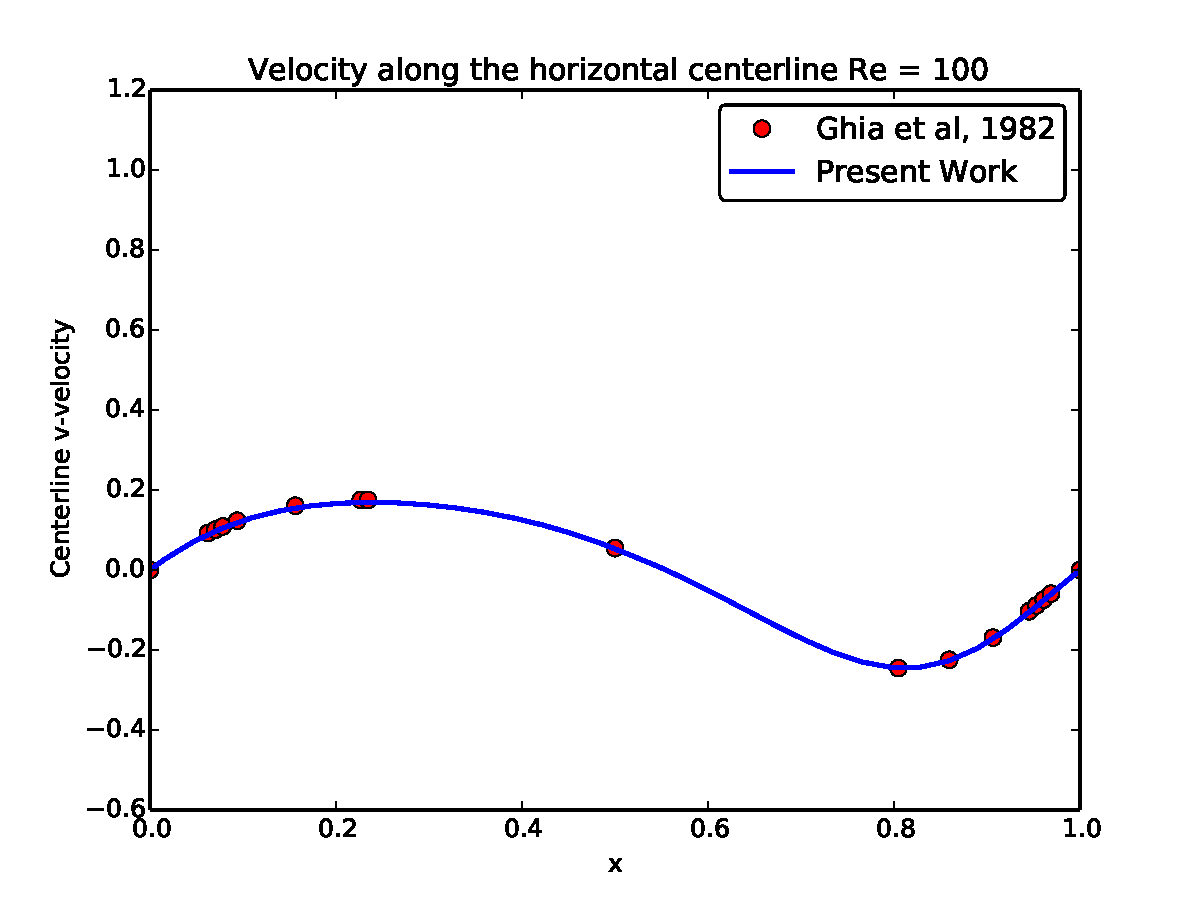
\includegraphics[width=\linewidth]{ldc_horizontal_100}
		\caption{Horizontal Centerline Re 100.}		
	\end{subfigure}
	~
	\begin{subfigure}{0.4\textwidth}
		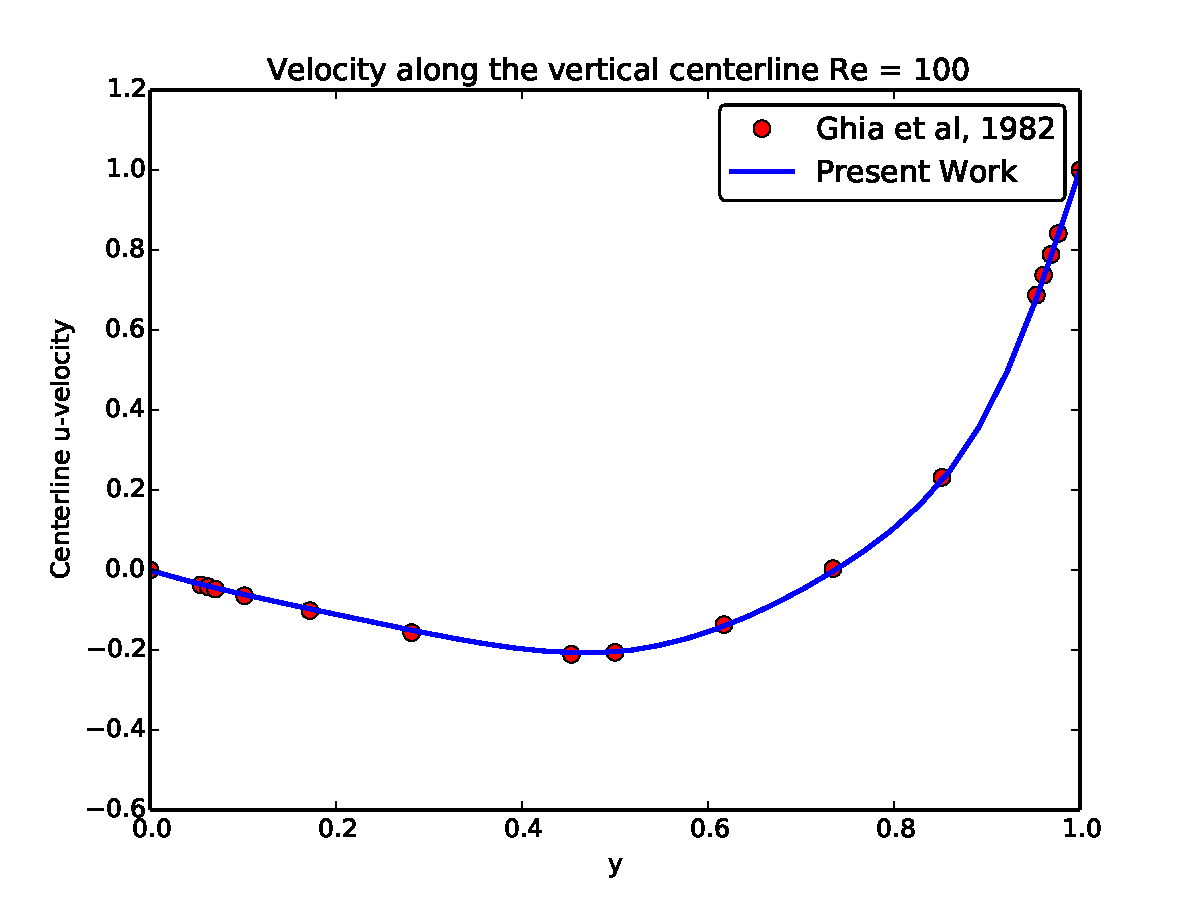
\includegraphics[width=\linewidth]{ldc_vertical_100}
		\caption{Vertical centerline Re 100.}		
	\end{subfigure}
	
	\begin{subfigure}{0.4\textwidth}
		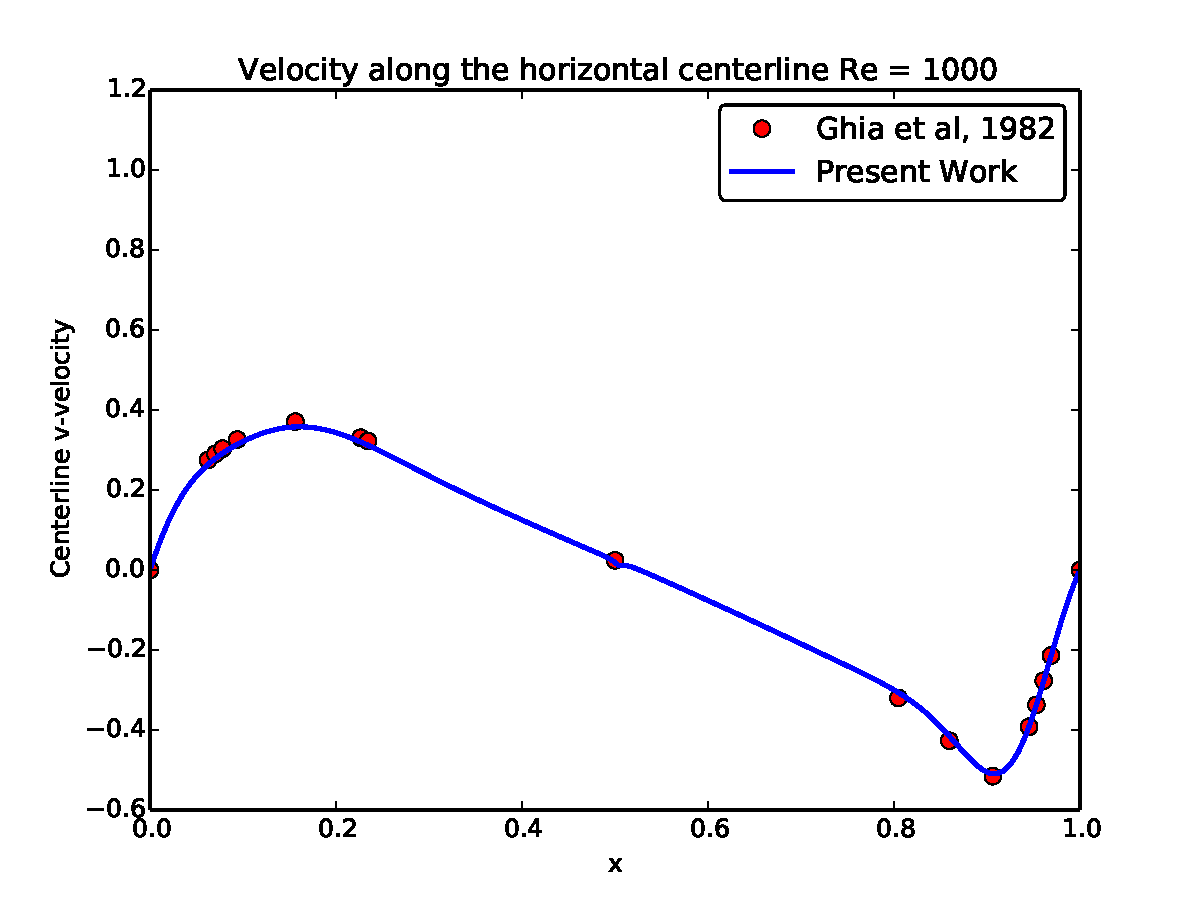
\includegraphics[width=\linewidth]{ldc_horizontal_1000}
		\caption{Horizontal centerline Re 1000.}		
	\end{subfigure}
	~
	\begin{subfigure}{0.4\textwidth}
		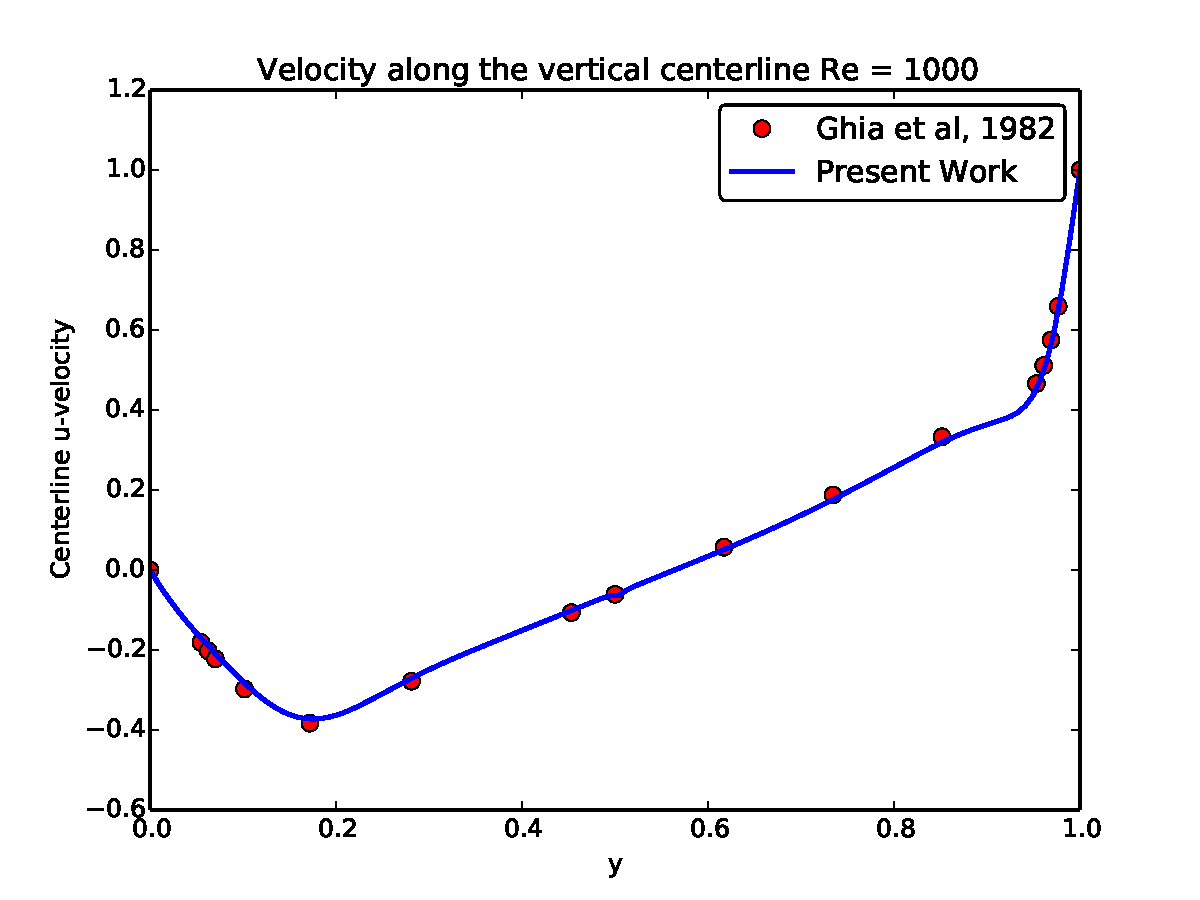
\includegraphics[width=\linewidth]{ldc_vertical_1000}
		\caption{Vertical centerline Re 1000.}		
	\end{subfigure}
	\caption{Verification for lid driven cavity. The top row is Re 100 and the bottom row is Re 1000. The left column is the $v$ velocity at the horizontal centerline and the right column is the $u$ velocity at the vertical centerline.}
	\label{fig:ldc}
\end{figure}

\section{Impulsively started cylinder}
\label{sec:cylinder}
The impulsively started cylinder simulation tests the IBMs' ability to handle an immersed body. 
It also tests the stretched grid and force calculation. 
This test mimics a body being 'impulsively started', as if it was struck by a hammer. 
In the first few time steps a very large sheer stress on the body will cause a high drag which rapidly dissipates and then slowly reaches steady state as the boundary layer develops and stabilizes. 
The IBM can be verified by plotting the drag over time and comparing to the results of Koumoutsakos and Leonard~\cite{Koumoutsakos:1995bf}. 
To simulate an impulsively started cylinder, a circular body is anchored to the origin and an initial $u$ velocity of one is set over the entire fluid domain. 
The left, top, and bottom boundaries have Dirichlet $u$ and $v$ values one and zero forming an inlet and two free stream boundaries. 
A convective boundary condition is used at right edge that uses one and zero for nominal $u$ and $v$ values. 
The grids are made up of uniform spacing in the area immediate around the immersed body that stretches as it moves away from the center until it reaches the domain's edge at $\pm$ 15. 
Figure~\ref{fig:iscylinder} shows the domain of the Reynolds number 40 simulation, the domains for Reynolds number 550 and 3000 have a slightly smaller uniform grid section in the middle. 
\begin{figure}[!htb]
	\centering
	\includestandalone[width=0.5\textwidth]{CylinderDomain}
	\caption{The domain of and impulsively started cylinder simulation with Reynolds number forty.}
	\label{fig:iscylinder}
\end{figure}

All lengths are normalized against the body diameter, i.e the circle's diameter is one.
For a Reynolds number of 40 a uniform grid with spacing 0.025 is used from (-0.6,-0.6) to (0.6,0.6) for a total of 186x186 cells are used.
\todo{find cfl number}
A time step of 0.005 is used with a maximum CFL of approximately.
Figure \ref{fig:cy40}a and \ref{fig:cy40}b compares the computed drag force of the modified Fadlun et al. and external Luo et al. methods respectively to that of Koumoutsakos and Leonard.
\begin{figure}[!htb]
	\centering
	\begin{subfigure}{0.4\textwidth}
		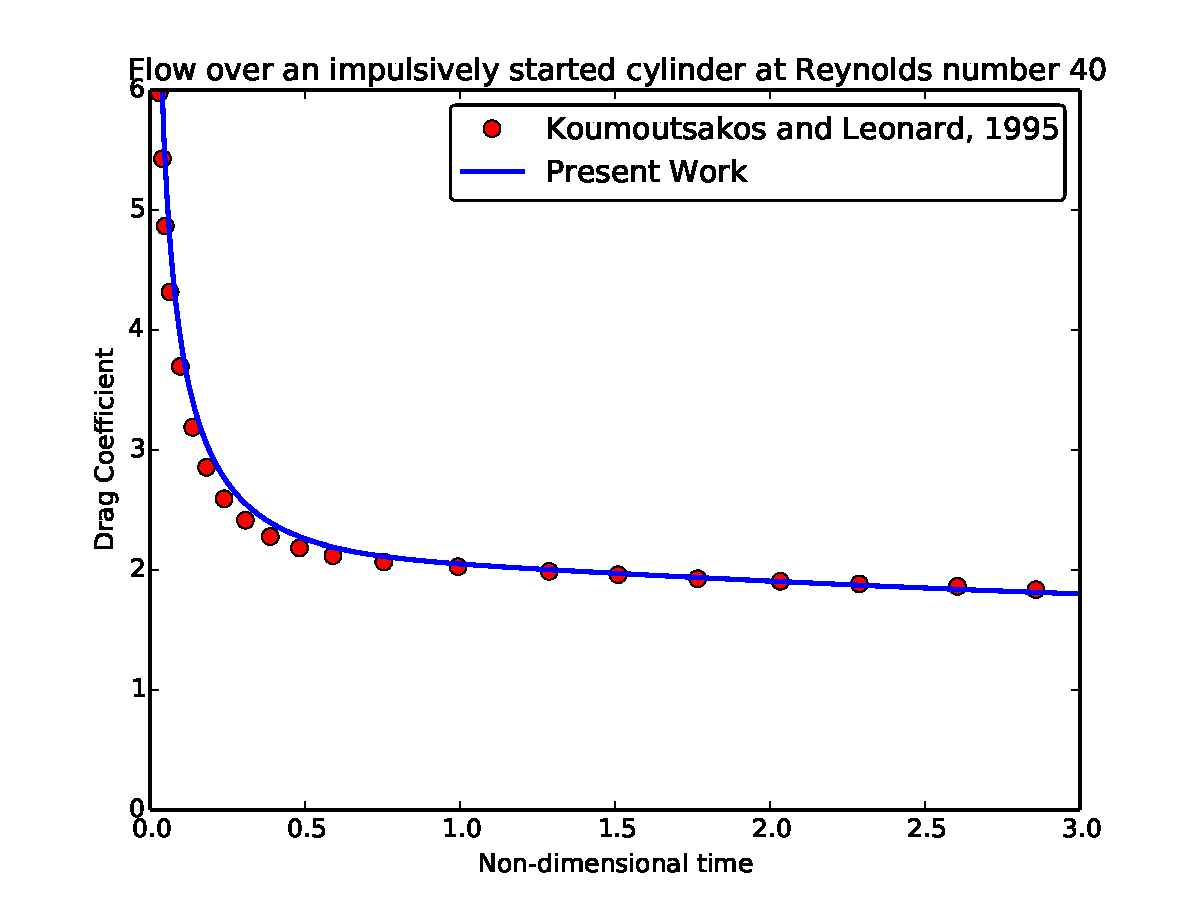
\includegraphics[width=\linewidth]{cy40fadlun}
		\caption{Modified Fadlun et al. style solver.}
	\end{subfigure}
	~
	\begin{subfigure}{0.4\textwidth}
		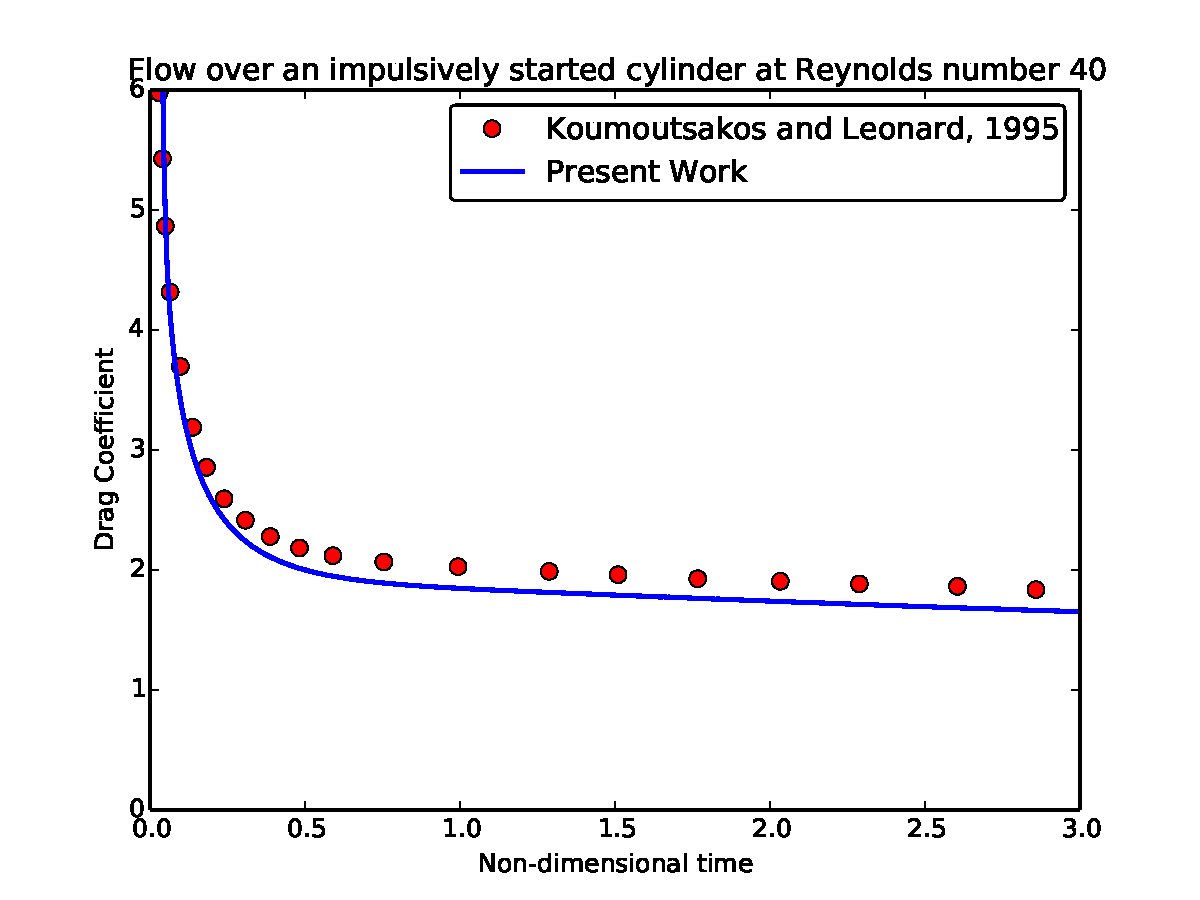
\includegraphics[width=\linewidth]{cy40luo}
		\caption{External Luo et al. style solver.}
	\end{subfigure}
	\caption{Drag force verses time for two solvers compared to Koumoutsakos and Leonard for flow over an impulsively started cylinder.}
	\label{fig:cy40}
\end{figure}

For a Reynolds number of 550 a uniform grid with spacing 0.01 is used from (-0.54,-0.54) to (0.54,0.54) for a total of 186x186 cells are used.\todo{update total grid size}
\todo{find cfl number}
A time step of 0.0025 is used for a maximum CFL number of.
Figure \ref{fig:cy550}a and \ref{fig:cy550}b compares the computed drag force of the modified Fadlun et al. and external Luo et al. methods respectively to that of Koumoutsakos and Leonard for a Reynolds number of 550
\begin{figure}[!htb]
	\centering
	\begin{subfigure}{0.4\textwidth}
		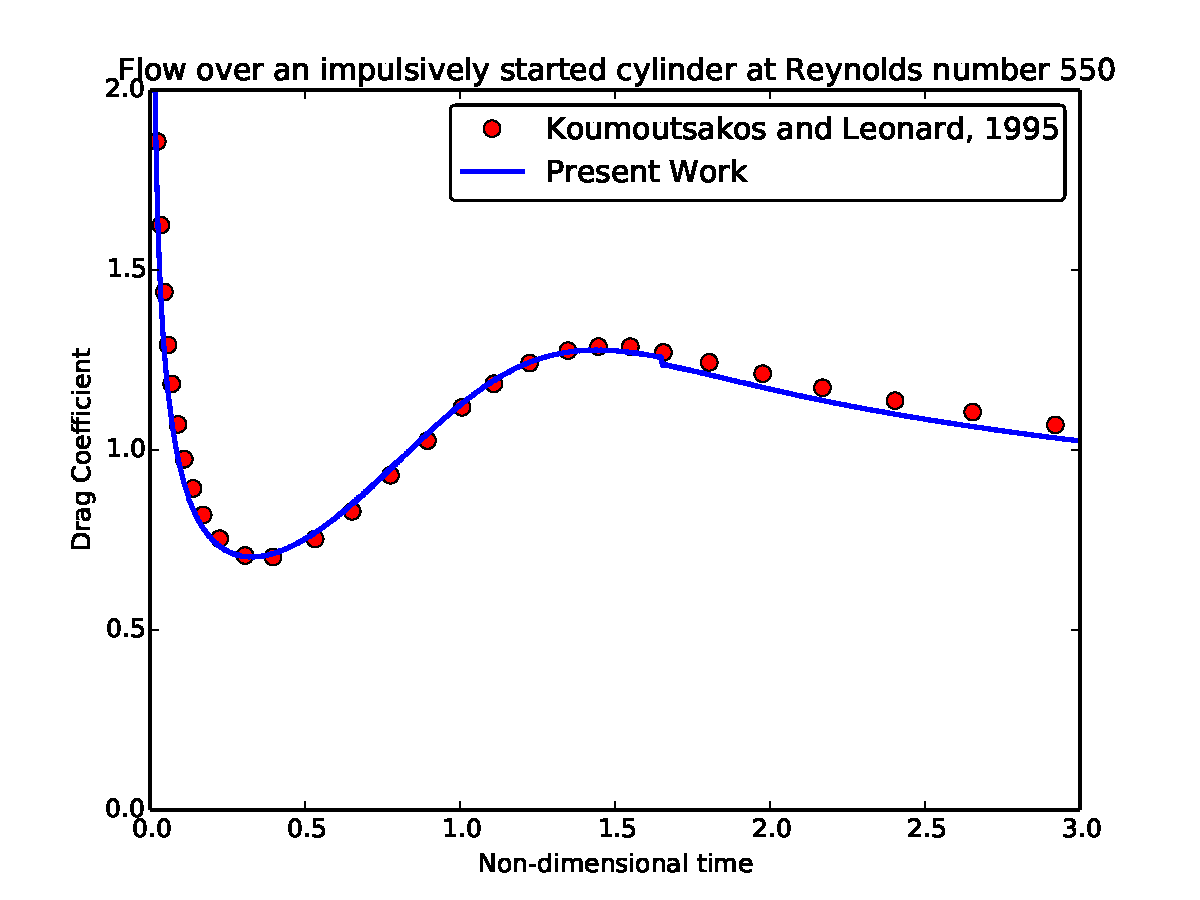
\includegraphics[width=\linewidth]{cy550fadlun}
		\caption{Modified Fadlun et al. style solver.}
	\end{subfigure}
	~
	\begin{subfigure}{0.4\textwidth}
		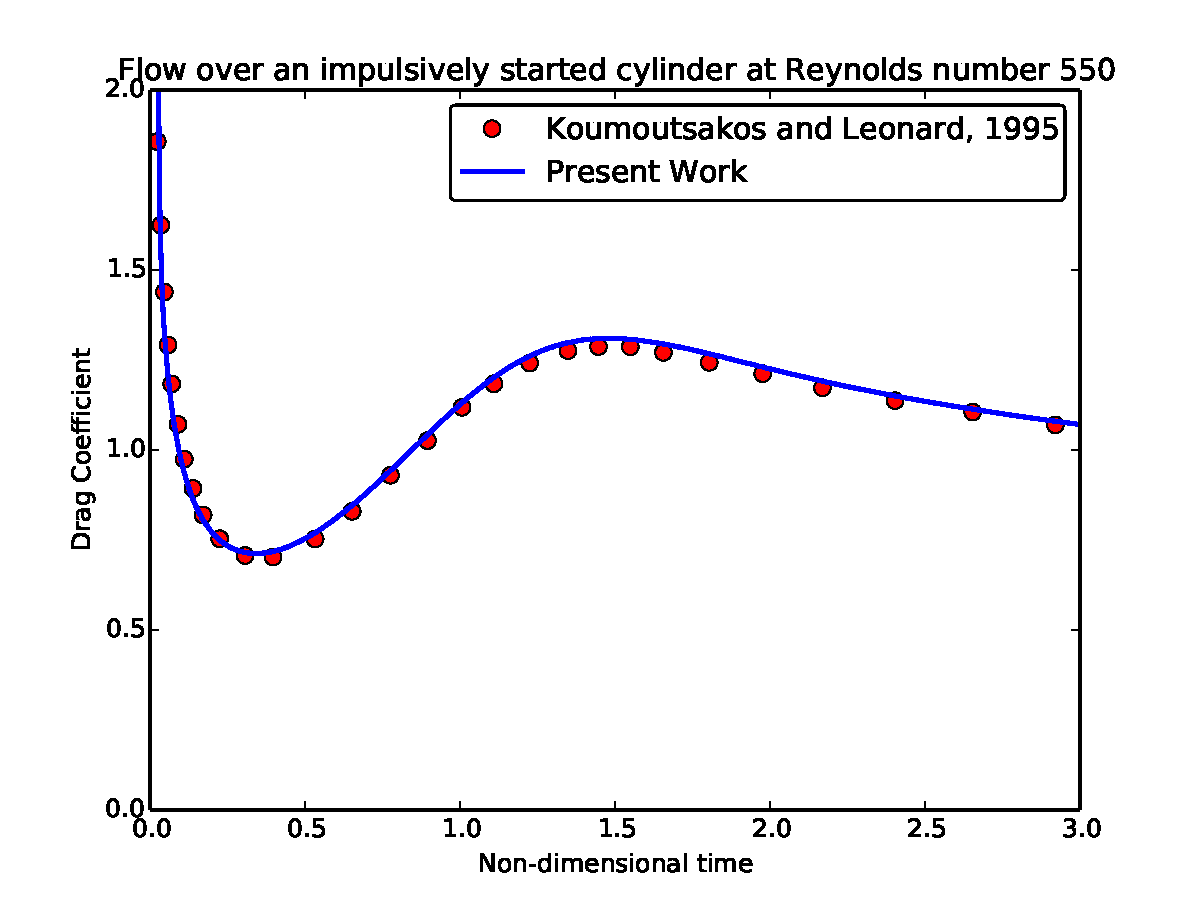
\includegraphics[width=\linewidth]{cy550luo}
		\caption{External Luo et al. style solver.}
	\end{subfigure}
	\caption{Drag force verses time for two solvers compared to Koumoutsakos and Leonard for flow over an impulsively started cylinder.}
	\label{fig:cy550}
\end{figure}

For a Reynolds number of 3000 a uniform grid with spacing 0.004 is used from (-0.52,-0.52) to (0.52,0.52) for a total of 186x186 cells are used.\todo{find correct size}
\todo{find cfl number}
A time step of 0.001 is used for a maximum CFL of.
Figure \ref{fig:cy3000}a and \ref{fig:cy3000}b compares the computed drag force of the modified Fadlun et al. external Luo et al. methods respectively to that of Koumoutsakos and Leonard for a Reynolds number of 3000.
\begin{figure}[!htb]
	\centering
	\begin{subfigure}{0.4\textwidth}
		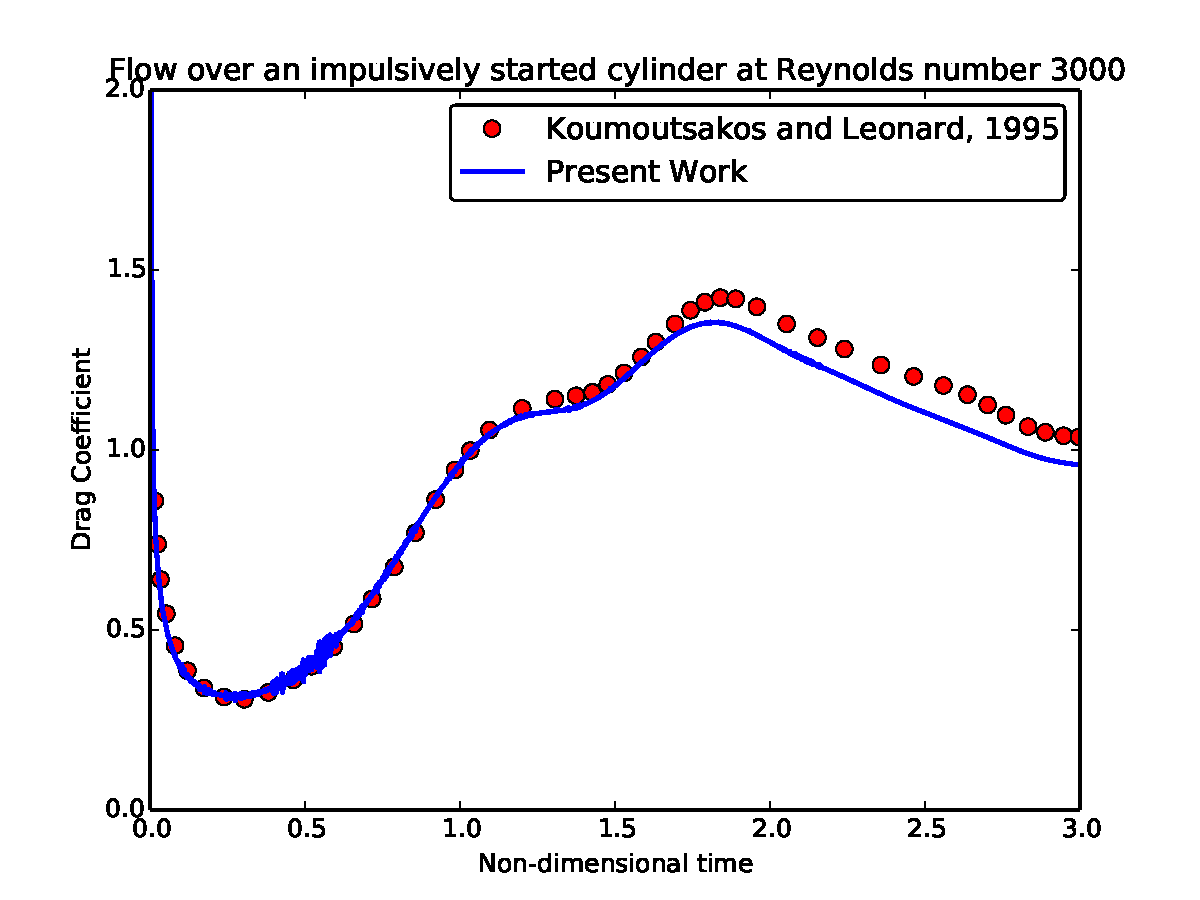
\includegraphics[width=\linewidth]{cy3000fadlun}
		\caption{Modified Fadlun et al. style solver.}
	\end{subfigure}
	~
	\begin{subfigure}{0.4\textwidth}
		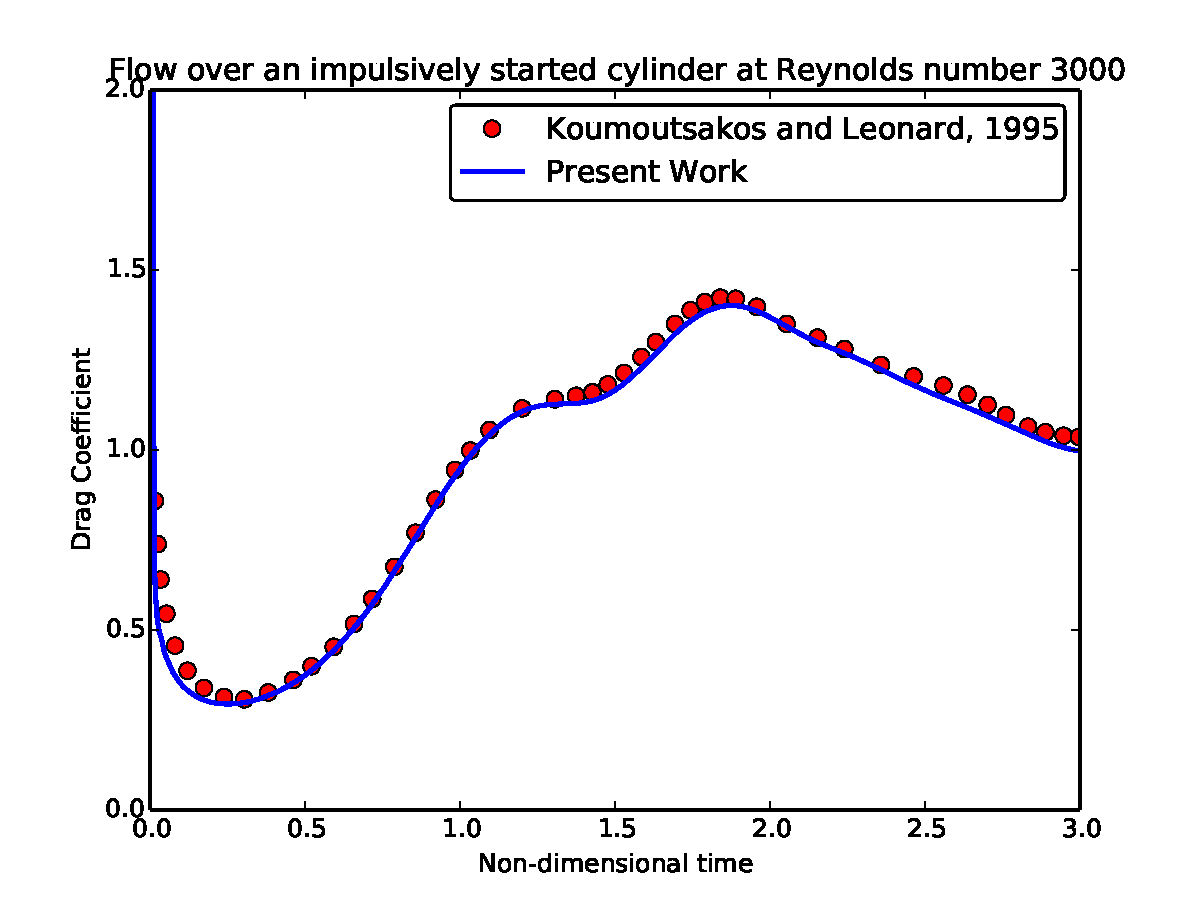
\includegraphics[width=\linewidth]{cy3000luo}
		\caption{External Luo et al. style solver.}
	\end{subfigure}
	\caption{Drag force verses time for two solvers compared to Koumoutsakos and Leonard for flow over an impulsively started cylinder.}
	\label{fig:cy3000}
\end{figure}

The very large drag at the beginning is caused by the impulsive start of the body.
At the first time step, when all the fluid nodes have a $u$ velocity of one, the $\frac{du}{dx}$ term of shear force is large as $du$ is still one and $dx$ is the small grid spacing.
It is interesting that neither method is consistently over or under predicting the correct drag.
Instead, both of them are changing based on time and Reynolds number.
Another result of note are the drag oscillations between 0.25 and 0.75 in the Re=3000 Fadlun results \ref{fig:cy3000}a.
The modified Fadlun method appears to undergo numerical oscillations when stressed, i.e. extreme Reynolds number, grid sizing or time step. 

\section{Flow past an in-line oscillating cylinder}
\label{sec:osccylinder}
The impulsively started oscillating cylinder is a simulation used by Luo et al\cite{Luo:2012gx}. to demonstrate and compare the magnitude numerical oscillations between different IBMs. 
It is not a verification or validation as it doesn't compare the results to published work, rather it is a useful tool to visualize the magnitude of numerical oscillations.
A true moving body verification is done in the next section,\ref{sec:Oscillating Cylinder in no Flow}
This simulation has the same domain, initial and boundary conditions as the stationary impulsively started cylinder save for the uniform grid at the center which spans from (-2,-2) to (2,2) to account for body's movement.
The cylinder oscillates along the horizontal centerline according to equations \eqref{eq:cylinder position} and \eqref{eq:cylinder velocity}.
The resulting period, maximum velocity and position are 5, $\pi/10$ and 0.25 respectively.
\begin{align}
x&=-0.25\cos{0.4\pi t}\label{eq:cylinder position}\\
u&=0.1\pi\sin{0.4\pi t}\;\label{eq:cylinder velocity}
\end{align}
Figure \ref{fig:osccylinder} compares the numerical oscillations seen in drag vs time. 
The left column shows drag force experienced the external method.
The right column shows the drag force experienced by the embedded method.
The uniform section is discretized into a $64 \times 64$ grid for the first row and $ 128 \times 128$ grid for last three rows row for h values of 0.0625 and 0.03125.
The maximum CFL numbers by row are approximately \numlist{0.35; 0.35; 0.7; 1.0}.
\begin{figure}[!htb]
	\centering
	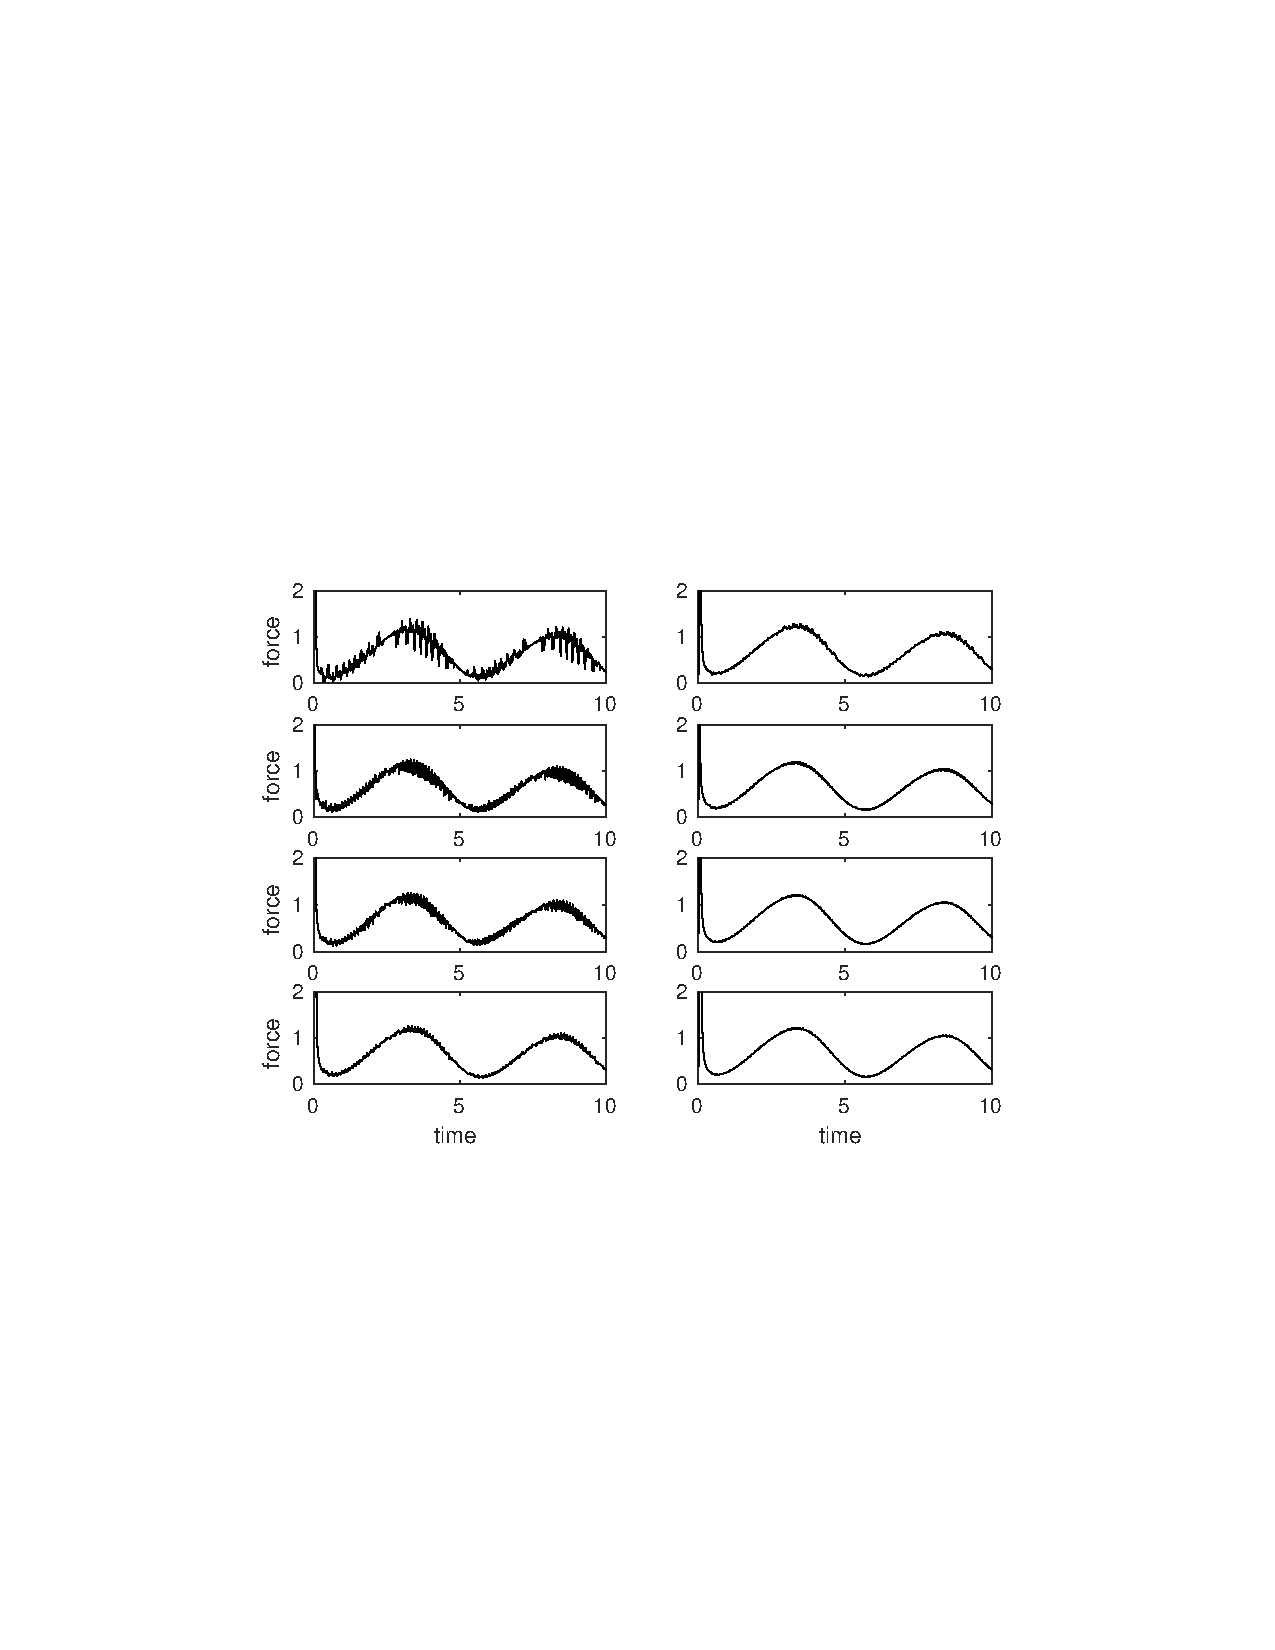
\includegraphics[width=\textwidth]{cropped_oscflow}
	\caption{The left column shows external interpolation and the right column shows the embedded interpolation. Rows one though four are maximum CFL \numlist{0.35; 0.35; 0.7; 1.0} and have a middle grid spacing of \numlist{0.0625; 0.0313; 0.0313; 0.0313}}
	\label{fig:osccylinder}
\end{figure}

Both methods suppress the magnitude of the oscillations by decreasing in grid size.
The frequency of the oscillations is also reduced by increasing the maximum CFL number.
This effect is most easily seen in the left column.
The embedded method, as expected, is better at suppressing oscillations than the external method.
If the bottom row is examined closely it can be seen that both methods only suppress the oscillations, not eliminate them.
It is interesting that, in spite of the oscillations, similar maximum force values could be obtained from any of the eight plots.
The accuracy of the two methods is examined in the next section.

\section{Oscillating Cylinder in no Flow}
\label{sec:Oscillating Cylinder in no Flow}
Oscillation of a cylinder in now flow is a simulation used by Liao et al~\cite{liao2010simulating}. to demonstrate numerical oscillation suppression. 
Liao et al. and cuIBM-FSI are validated against the experimental data of Dutsch et al~\cite{dutsch1998low}.
The equations that govern movement, \ref{eq:cylinder position2} and \ref{eq:cylinder velocity2}, are the same form as above but with a period, maximum velocity and position of 1, 1 and $1/2\pi$.
The diameter is matched to the Liao et al. simulation which is 0.2. 
The domain has uniform section with grid spacing 0.005 from (-0.4,-0.2) to (0.4,0.2). 
It ranges from $\pm$ 5.5 in the x to $\pm$ 3.5 in the y. 
A Reynolds number of 100 and a KC number(non-dimensional number that represents the bodies oscillation) of 5 is used.
\begin{align}
x&=\frac{-1}{2\pi}\sin{2\pi t}\label{eq:cylinder position2}\\
u&=-cos{2\pi t}\;\label{eq:cylinder velocity2}
\end{align}

Figure \ref{fig:staticInit} shows the drag during the first period versus the steady state drag from Liao et al. 
Figure \ref{fig:static2} shows the steady state drag.
In both figures, (a) is the external method and (b) is the embedded method.
 
\begin{figure}[!htb]
	\centering
	\begin{subfigure}{0.4\textwidth}
		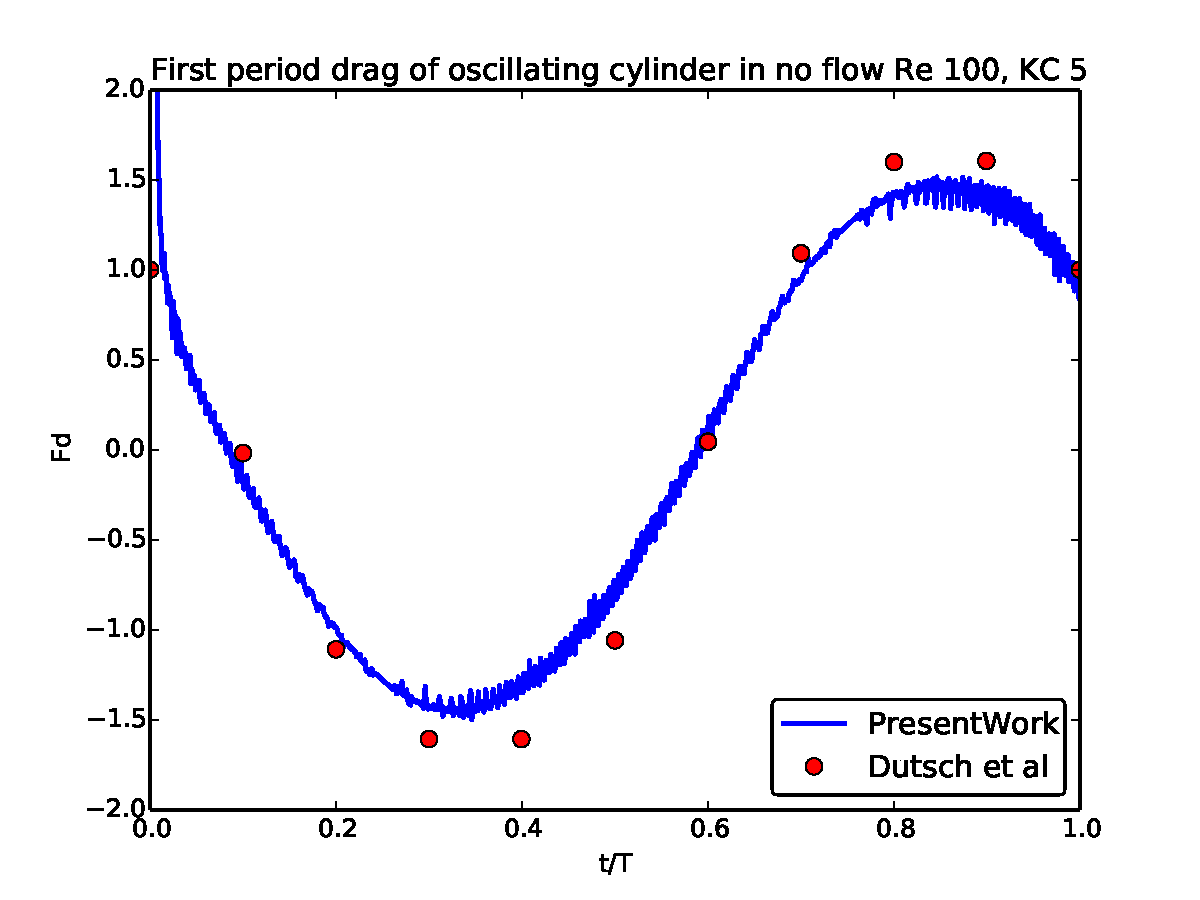
\includegraphics[width=\linewidth]{staticexinit}
		\caption{External interpolation method.}
	\end{subfigure}
	~
	\begin{subfigure}{0.4\textwidth}
		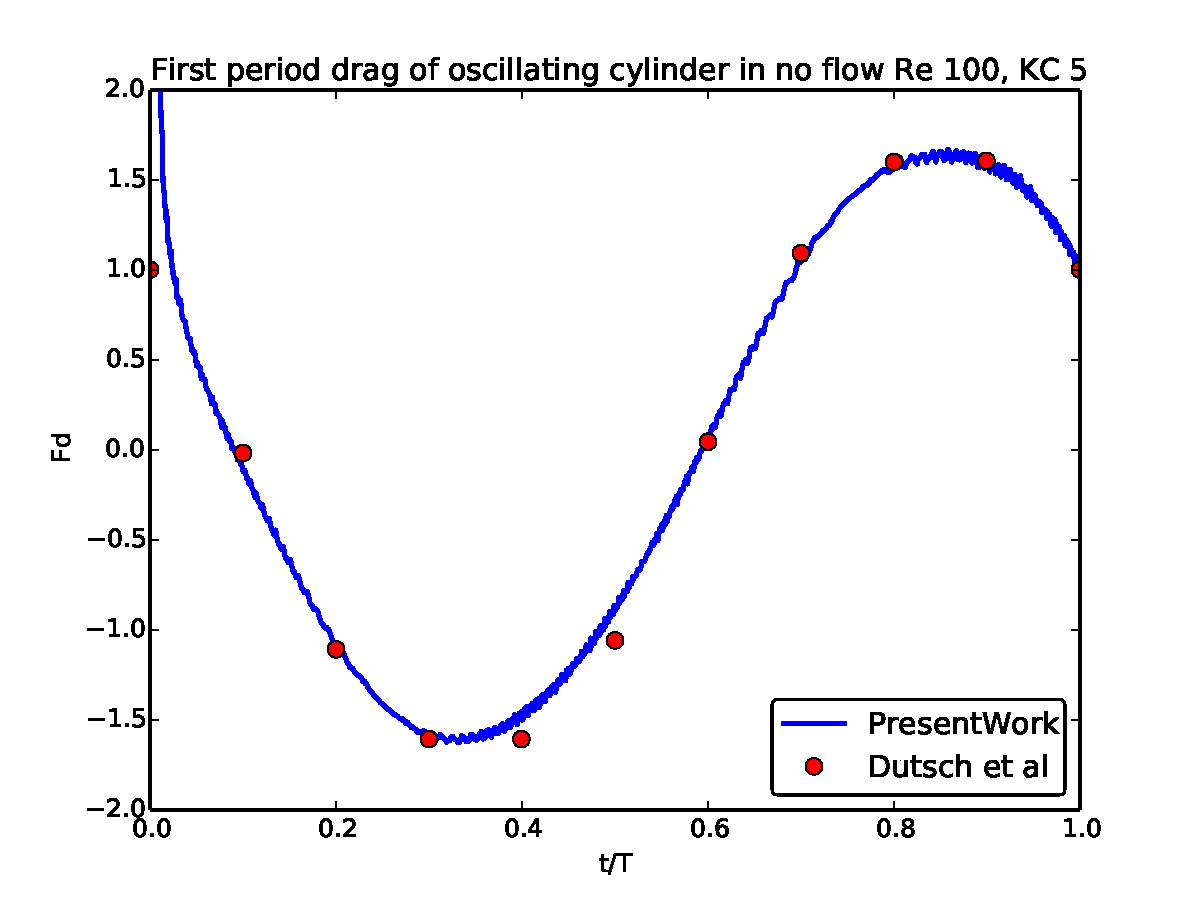
\includegraphics[width=\linewidth]{staticeminit}
		\caption{Embedded interpolation method.}
	\end{subfigure}
	\caption{Drag force verses time for the first period compared to steady state Liao et al. for an oscillating cylinder in no flow.}
	\label{fig:staticInit}
\end{figure}

\begin{figure}[htb]
	\centering
	\begin{subfigure}{0.4\textwidth}
		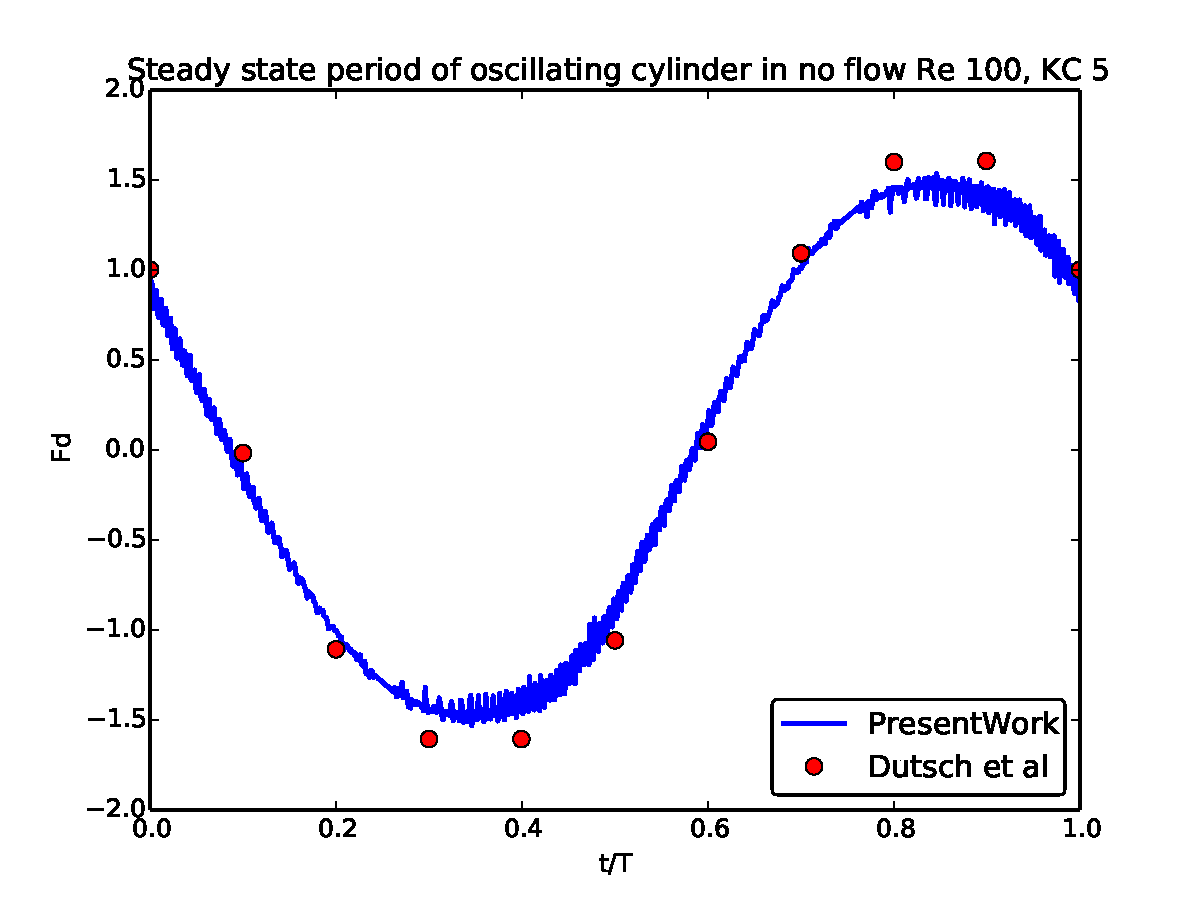
\includegraphics[width=\linewidth]{staticexss}
		\caption{External interpolation method.}
	\end{subfigure}
	~
	\begin{subfigure}{0.4\textwidth}
		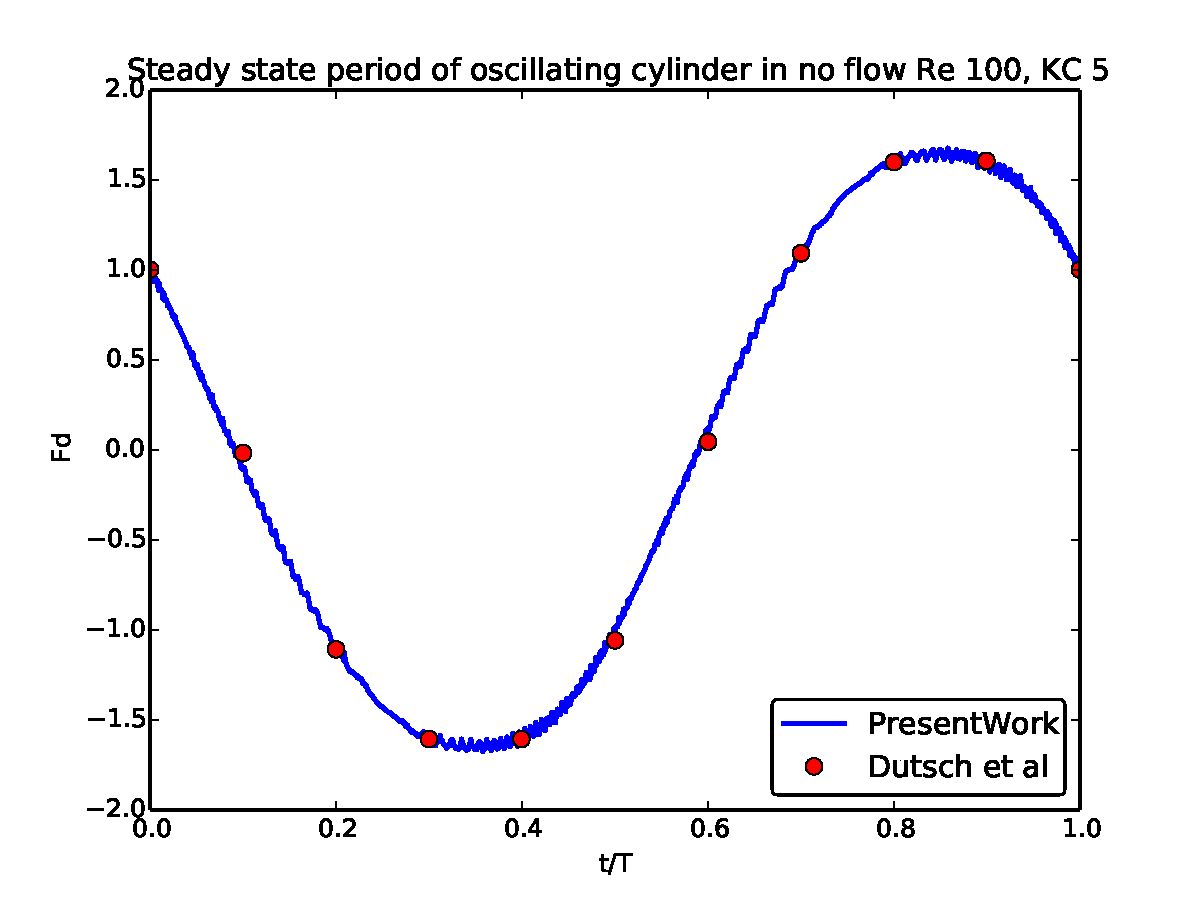
\includegraphics[width=\linewidth]{staticemss}
		\caption{Embedded interpolation method.}
	\end{subfigure}
	\caption{Drag force verses time for steady state oscillating cylinder in now flow compared to Liao et al.}
	\label{fig:static2}
\end{figure}

Again the embedded solver is doing a better job at supressing the oscillations. It is also better predicting the maximum peak than the external method, which is about 15\% off of the experimental data.

\section{Vorticity Induced Vibration}
The vorticity induced vibration simulation tests the solvers ability to predict the position of a freely moving body in coupled fluid structure interaction.
The domain is the same as the impulsively started cylinder simulation except the uniform region ranges from -1.5 to 1.5 and -1.5 to 1.5 in the x and y respectively.
An immersed circle starts at the origin with no initial velocity. 
The body is free to move in the y direction but fixed in the x and is mounted to a spring to prevent it from wandering off. 
In VIV the Reynolds number is set in a range that sheds oscillating vortices, in this case it's 150. 
This combined with the spring causes the body to establish a steady state sinusoidal motion for which the amplitude can be verified with literature.
Following the work of Borazjani et al\cite{borazjani2008curvilinear}. the mass spring damper system \eqref{eq:masspring} that governs the body's movement is non-dimensionalized to become equation \eqref{eq:ndmasspring}. 
\begin{equation}
M\frac{\partial^2Y}{\partial t^2}+C\frac{\partial Y}{\partial t}+KY=F_y \label{eq:masspring}
\end{equation}
$Y$ is the center coordinate of the body, $M$ is the mass, $C$ is the damping factor, $K$ is the stiffness and $F_y$ is the total fluid force on the body in the y direction. 
The natural frequency and critical damping are given by \eqref{eq:nf} and \eqref{eq:cd}. 
\begin{align}
\omega &=2\pi f =\sqrt{\frac{K}{M}}\label{eq:nf}\\
C_{cr}&=2\sqrt{MK}=2K\omega \; \label{eq:cd}
\end{align}
\begin{equation}
\frac{\partial^2 Y}{\partial t^2}+4\pi \zeta\frac{1}{U_{red}}\frac{\partial Y}{\partial t}+4\pi^2\frac{1}{u_{red}^2}Y=\frac{1}{2M_{red}}C_Y\label{eq:ndmasspring}
\end{equation}
Borazjani et al. defines the non-dimensional coefficients as follows:\newline
Damping coefficient
\begin{equation}
\zeta=\frac{C}{C_{cr}}\label{eq:damping coefficient}
\end{equation}
Reduced velocity
\begin{equation}
U_{red}=\frac{U}{fD}\label{eq:reduced velocity}
\end{equation}
Reduced mass
\begin{equation}
M_{red}=\frac{M}{\rho D^2}\label{eq:reduced mass}
\end{equation}
Force coefficient
\begin{equation}
C_Y=\frac{2F_Y}{\rho U^2 D}\label{eq:force coefficient}
\end{equation}
Changing the parameters, Re, $\zeta$, $M_{red}$ and $U_{red}$ changes the resulting steady state amplitude. 
In VIV there is a 'lock-in' phenomenon that occurs when Re is set to 150, $\zeta$ is set to 0, $M_{red}$ is set to 2 and $U_{red}$ is varied between 3 and 8. 
At either extreme for $U_{red}$ the steady state amplitude will be small and for all the middle values the steady state amplitude will be much larger. 

There are two different ways to update body position, loose and strong coupling. 
Loose coupling comes from the explicit derivation of equation \eqref{eq:ndmasspring}.
A time step using loose coupling looks as follows:
\begin{enumerate}
	\item Solve for field values at $t^{n+1}$ using Naiver--Stokes.
	\item Calculate body forces.
	\item Move body using equations \eqref{eq:lc1} and \eqref{eq:lc2}.
\end{enumerate}
\begin{align}
v^{n+1} &= v^n-\frac{dt\pi^24}{U_{red}^2}\left(y^n+\frac{dtv^n}{2}\right) + \frac{dtC_Y}{\left(2M_{red}\right)\left(1+\frac{4dt^2\pi^2}{U_{red}^2}\right)} \label{eq:lc1} \\
y^{n+1} &= y^n +\frac{dt\left(v^{n+1}+v^n\right)}{2}\; \label{eq:lc2}
\end{align}

Equation \eqref{eq:ndmasspring} can also be discretized implicitly.
This is know as strong coupling.
A strong coupling time step repeatly calculates the field values and body kinetics/kinematics until a solution is converged on.
As this causes the Poisson equation to be solved multiple times for each time step resulting is a significantly more computationally expensive method:
\begin{enumerate}
	\item Solve for field values at sub step $t^{k+1}$ using Naiver--Stokes.
	\item Calculate body forces
	\item Move body using equations \eqref{eq:lc1} and \eqref{eq:sc} where $\alpha$ is some relaxation coefficient.
	\item If $|Y^{k+1}-Y^k| \approx 0$ advance time, otherwise advance sub step.
\end{enumerate}
\begin{equation}
y^{k+1} = \alpha \left(y^n+\frac{dt\left(v^{k+1}+v^n\right)}{2}\right) +\left(1-\alpha\right)y^k\label{eq:sc}
\end{equation}

Figures \ref{fig:viv1}, \ref{fig:viv2}, \ref{fig:viv3} and \ref{fig:viv4} show the maximum amplitude of the 6 VIV simulations as calculated by external loose coupling, external strong coupling, embedded loose coupling and embedded strong coupling respectively.
Results are verified against the curvilinear immersed boundary method of Borazjani et al.\cite{borazjani2008curvilinear} and the unstructured finite-element ALE approach of Ahn and Kallinderis\cite{ahn2006strongly}.
\begin{figure}
	\centering
	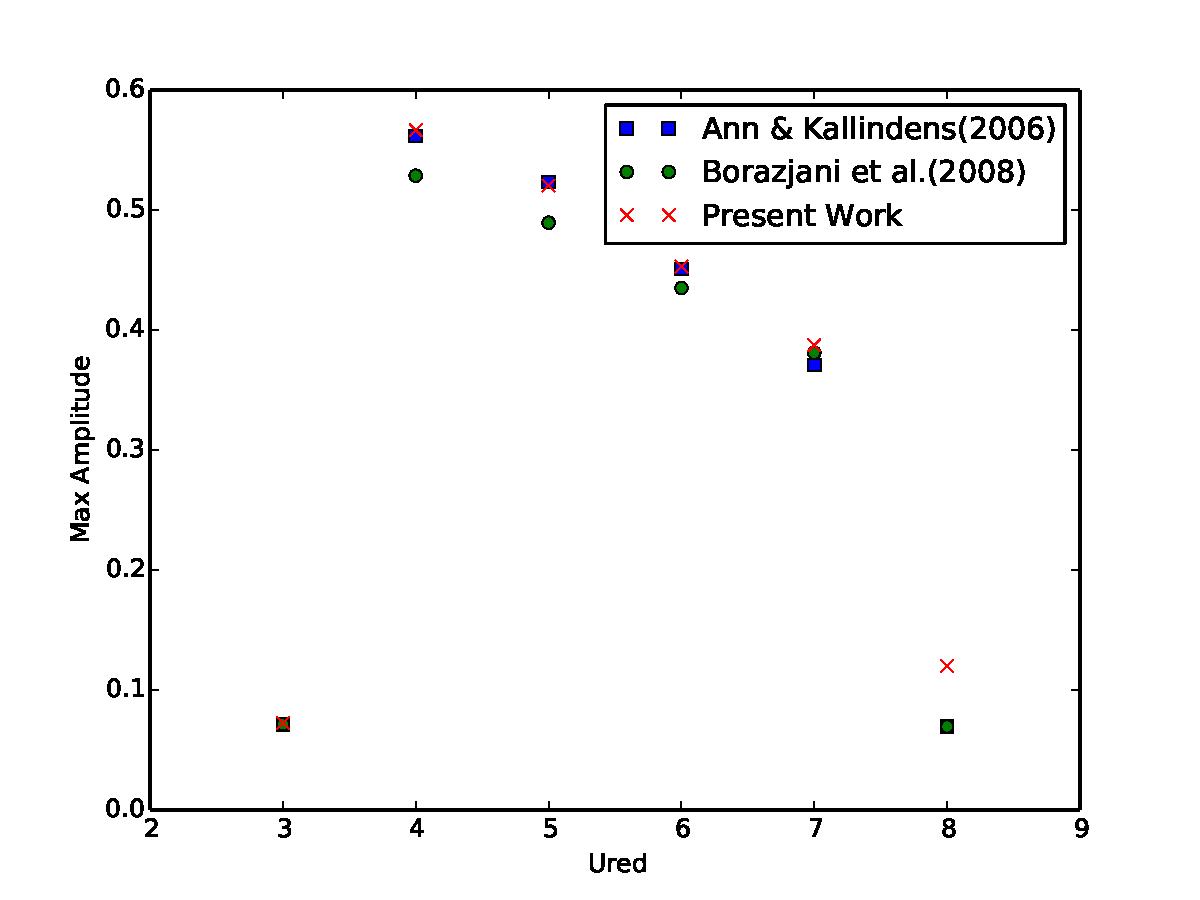
\includegraphics[width=\textwidth]{vivexlc}
	\caption{The maximum amplitude vs reduced velocity for the VIV lock in region calculated with external interpolation and loose coupling.}
	\label{fig:viv1}
\end{figure}
\begin{figure}
	\centering
	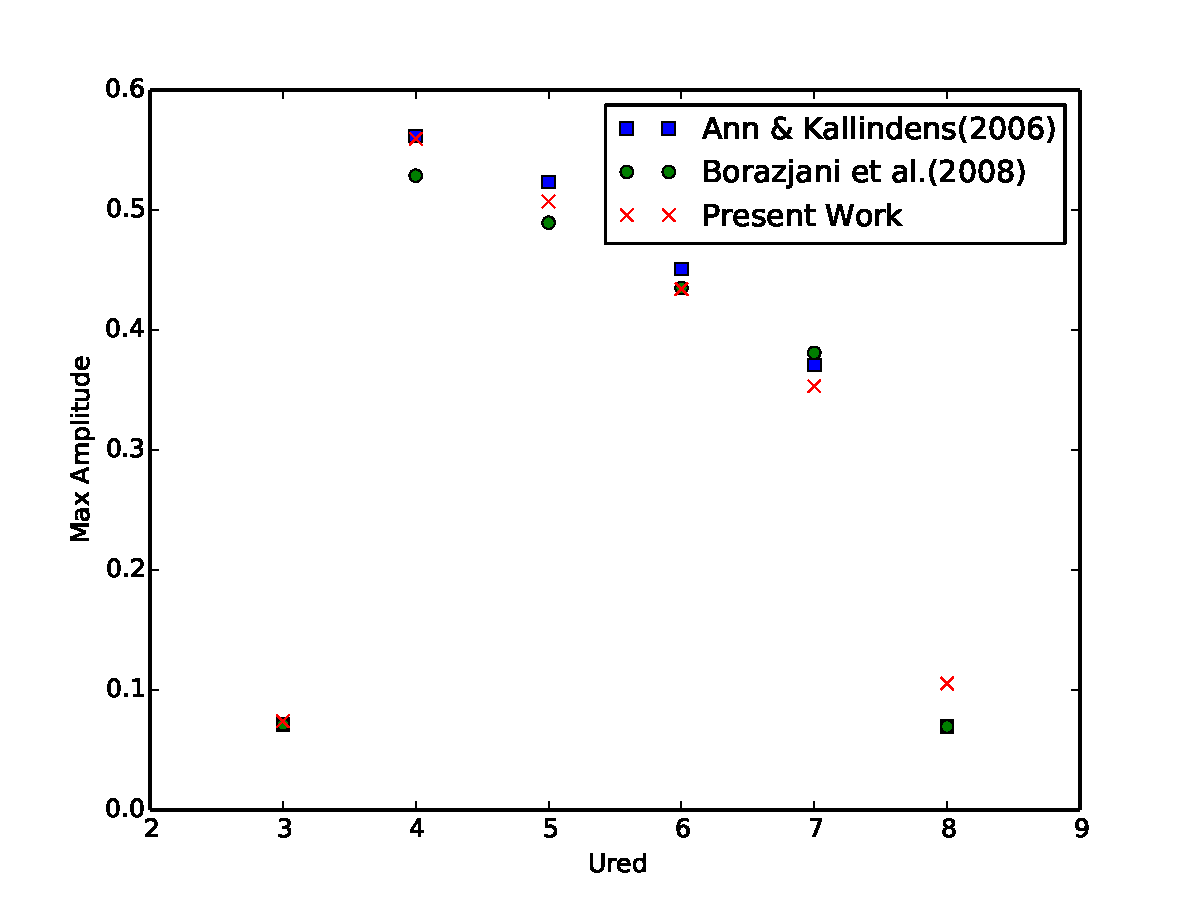
\includegraphics[width=\textwidth]{vivexsc}
	\caption{The maximum amplitude vs reduced velocity for the VIV lock in region calculated with external interpolation and strong coupling.}
	\label{fig:viv2}
\end{figure}
\begin{figure}
	\centering
	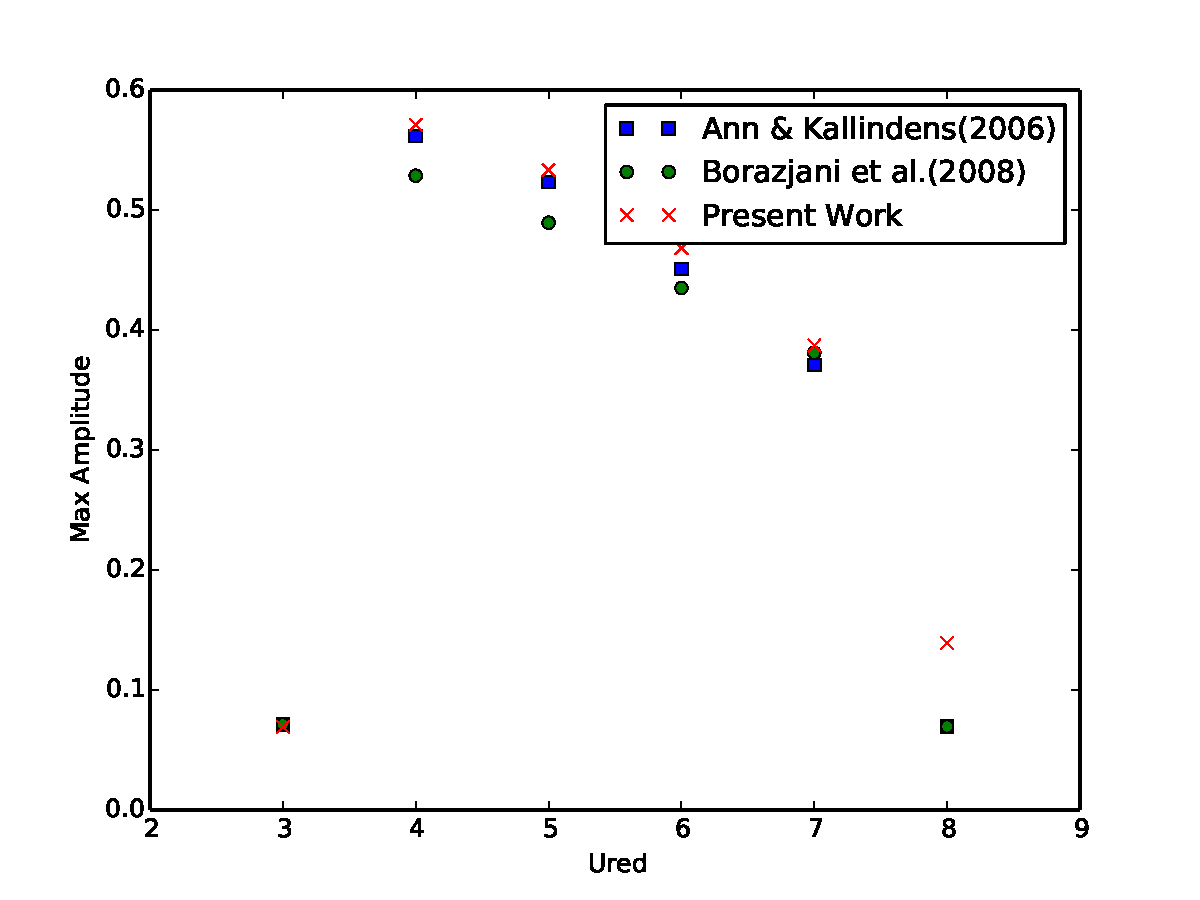
\includegraphics[width=\textwidth]{vivemlc}
	\caption{The maximum amplitude vs reduced velocity for the VIV lock in region calculated with embedded interpolation and loose coupling.}
	\label{fig:viv3}
\end{figure}
\begin{figure}
	\centering
	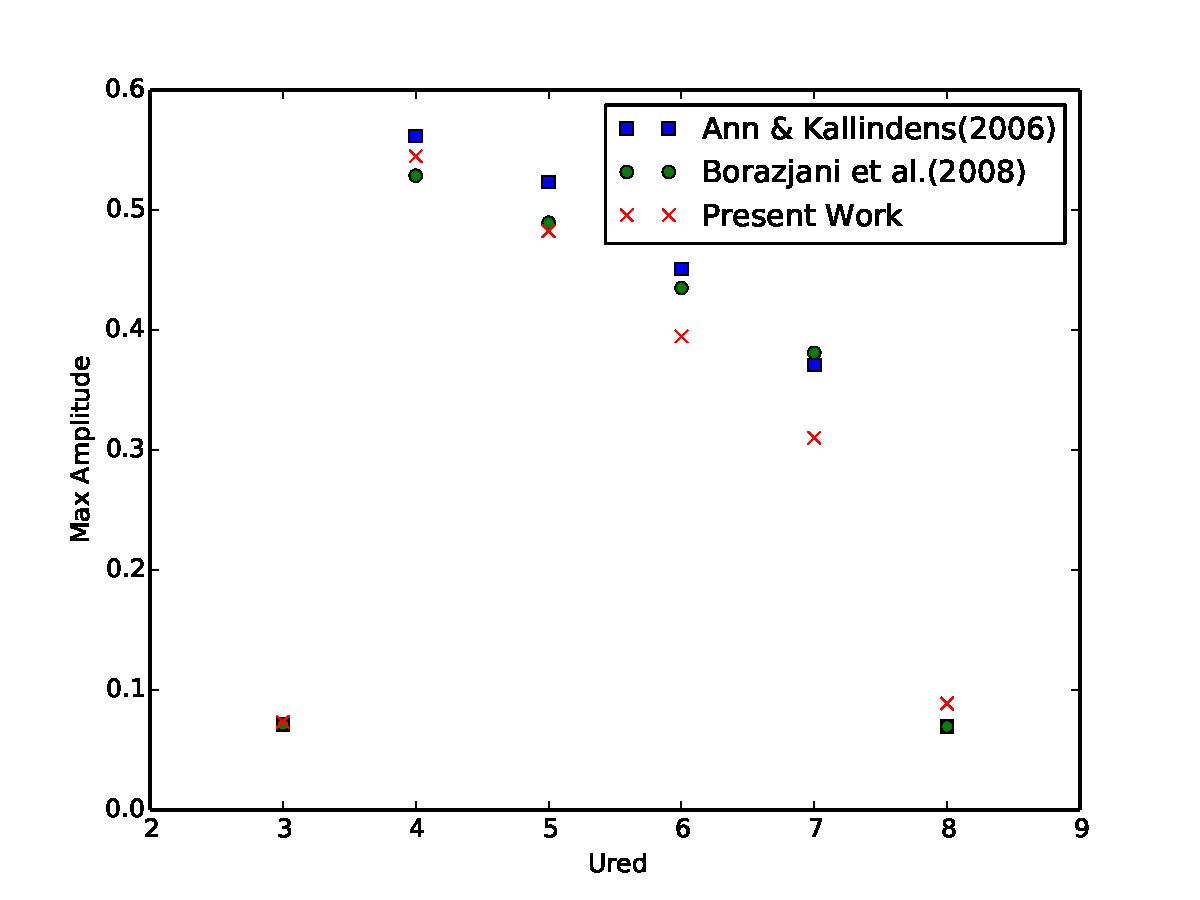
\includegraphics[width=\textwidth]{vivemsc}
	\caption{The maximum amplitude vs reduced velocity for the VIV lock in region calculated with embedded interpolation and strong coupling.}
	\label{fig:viv4}
\end{figure}

\chapter{Solver Characterization}
\label{chapter:error}
This section will evaluate the different methods used in terms of order of accuracy and performance scaling. 
The modified Fadlun, external and embedded methods will be evaluated using the impulsively started cylinder simulation and the external and embedded methods will be evaluated again using an oscillating cylinder in flow.

\section{Order of Accuracy}
Order of accuracy is evaluated by using a simulation evaluated with a fine grid as the 'exact' solution.
Coarser grids have their error calculated using the exact solution and are plotted on a log scale to see effects of grid size on accuracy.

\subsection{Impulsively started cylinder}
All grid sizes will refer to the grid spacing in the middle, which is uniform.
Grid spacings of \numlist{0.005; 0.005; 0.01} are used as the exact solution for the modified Fadlun, external and embedded impulsively started cylinder test. 
Using a different exact grid size for the embedded results to not be directly comparable but using a finer grid proved to make the solver unstable.
The reason for this is discussed below.
Three coarser grids with spacing ranging from 0.0625 to 0.01 have error calculated using the drag coefficient plotted in Figure~\ref{fig:cyerror}.
\begin{figure}[!htb]
	\centering
	\begin{subfigure}{0.3\textwidth}
		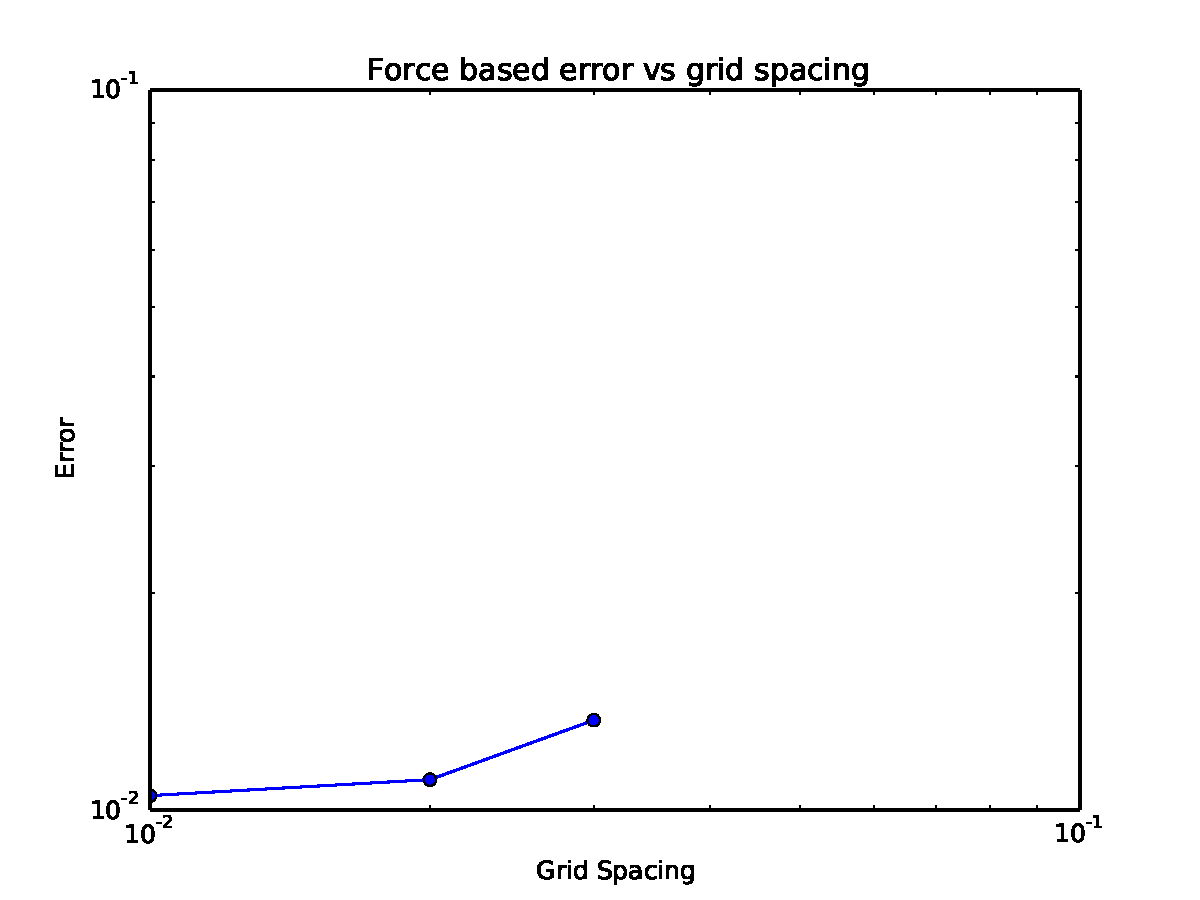
\includegraphics[width=\linewidth]{error_fadlun}
		\caption{Modified Fadlun}
	\end{subfigure}
	~
	\begin{subfigure}{0.3\textwidth}
		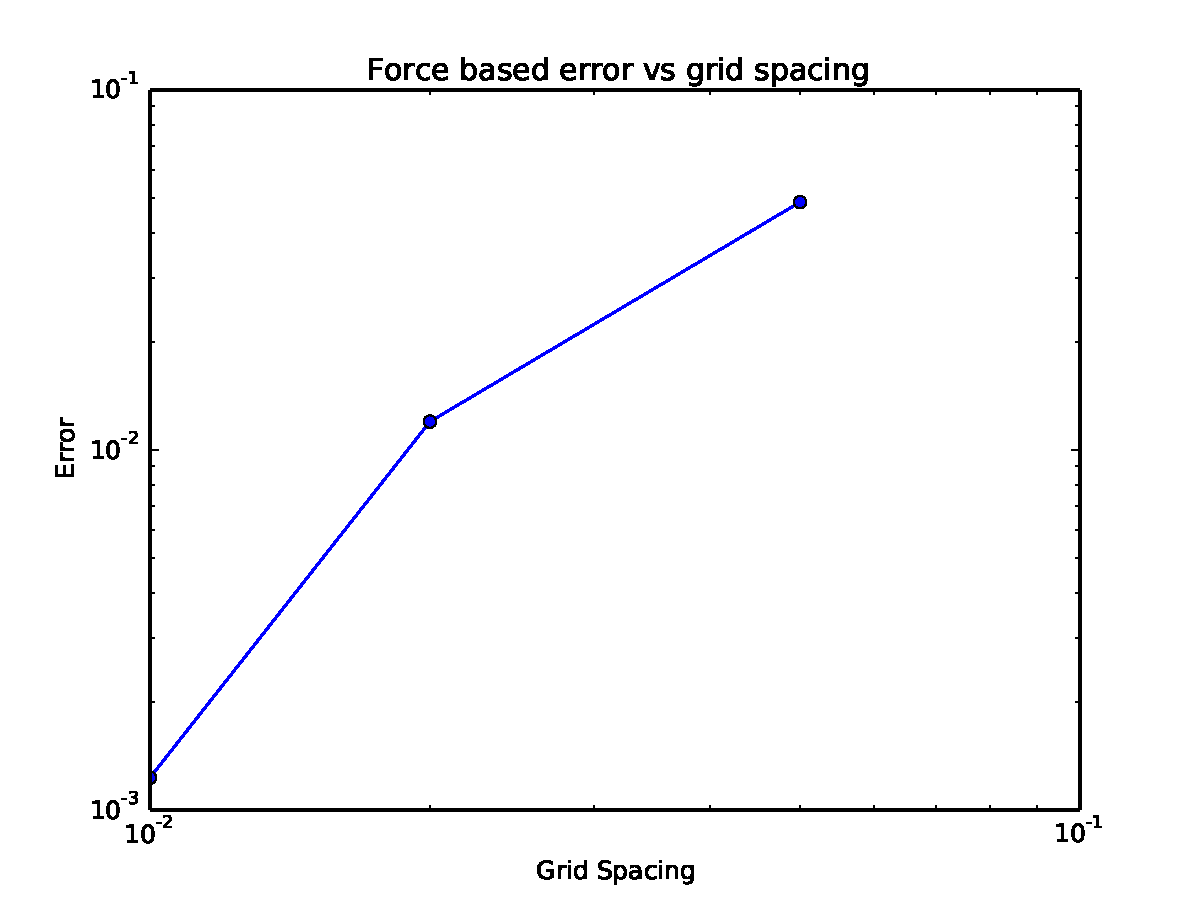
\includegraphics[width=\linewidth]{error_external}
		\caption{External}
	\end{subfigure}
	~
	\begin{subfigure}{0.3\textwidth}
		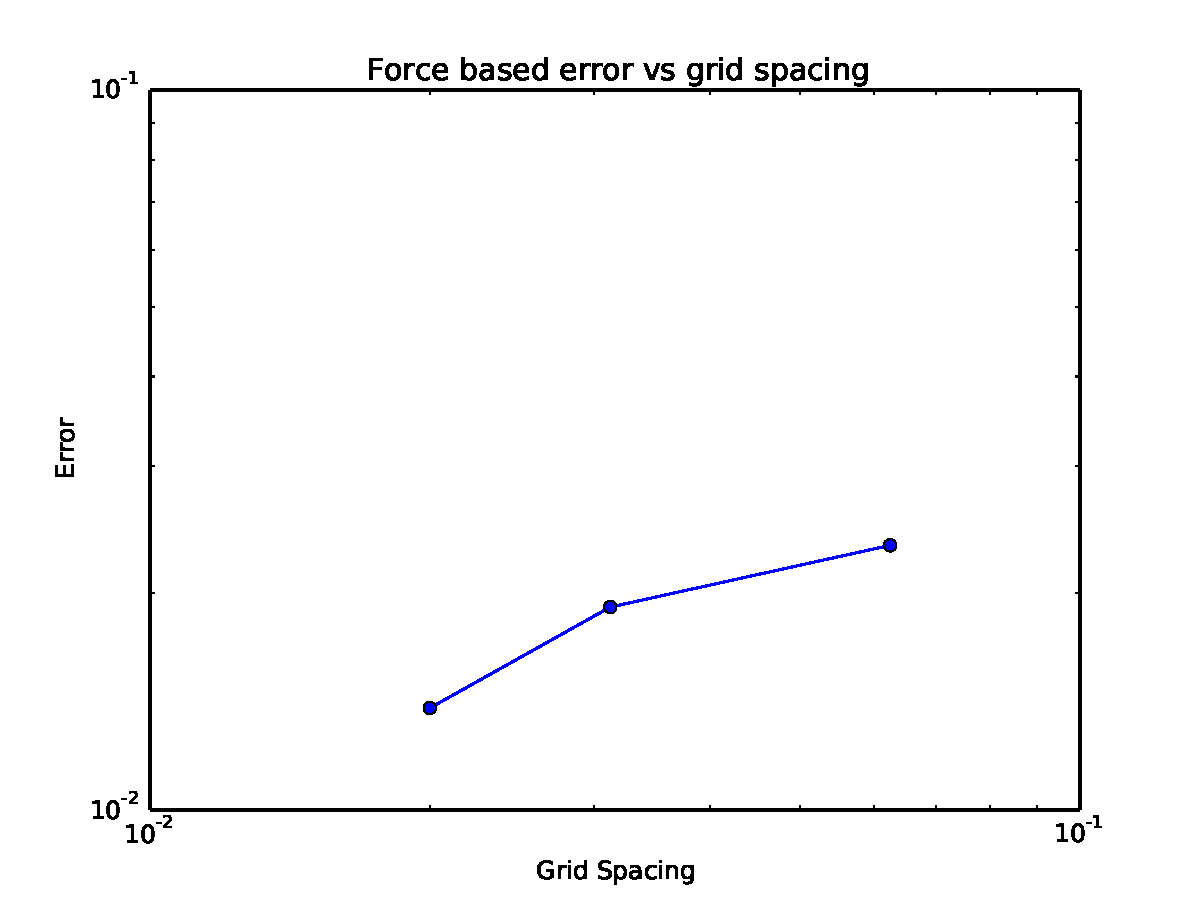
\includegraphics[width=\linewidth]{error_embedded}
		\caption{Embedded}
	\end{subfigure}
	\caption{Average error in drag force plotted against grid spacing shows the order of accuracy for the three solvers.}
	\label{fig:cyerror}
\end{figure}

The external method shows an order of accuracy around two but the modified Fadlun and embedded methods appear to not become more accurate with decreasing grid size. 
To explain this why they are not improving the individual results must be examined. 
Let's start with embedded method. 
Figure~\ref{fig:embedded005} shows the drag force of the two finest grid spacings, those corresponding with the exact solution and the left grid point of Figure~\ref{fig:cyerror}c. 
Using a grid spacing of 0.01 produces a small discontinuity at time 0.3 that none of the coarser grids have. 
The force error of grid size 0.015625 is plotted in Figure~\ref{fig:embeddederror005}. 
The error is dominated by the discontinuity after time 0.3 which causes poor order of accuracy results for the embedded method. 
If the error had stayed around the same magnitude before and after time 0.3 the average error would have worked out to be around 0.005 instead of the 0.015 plotted above. 
It is possible that the discontinuity is a real physical effect that the finer grid is capturing like a boundary layer reattaching to the body. 
It was not obvious what was causing the discontinuity by looking at velocity and pressure contours before and after the jump. 
This, coupled with the lack of a discontinuity present in the external method suggests it could be a numerical nuance. 
However, the effect is also present in the modified Fadlun method, just at a different time.

\begin{figure}[!htb]
	\centering
	\begin{subfigure}{0.4\textwidth}
		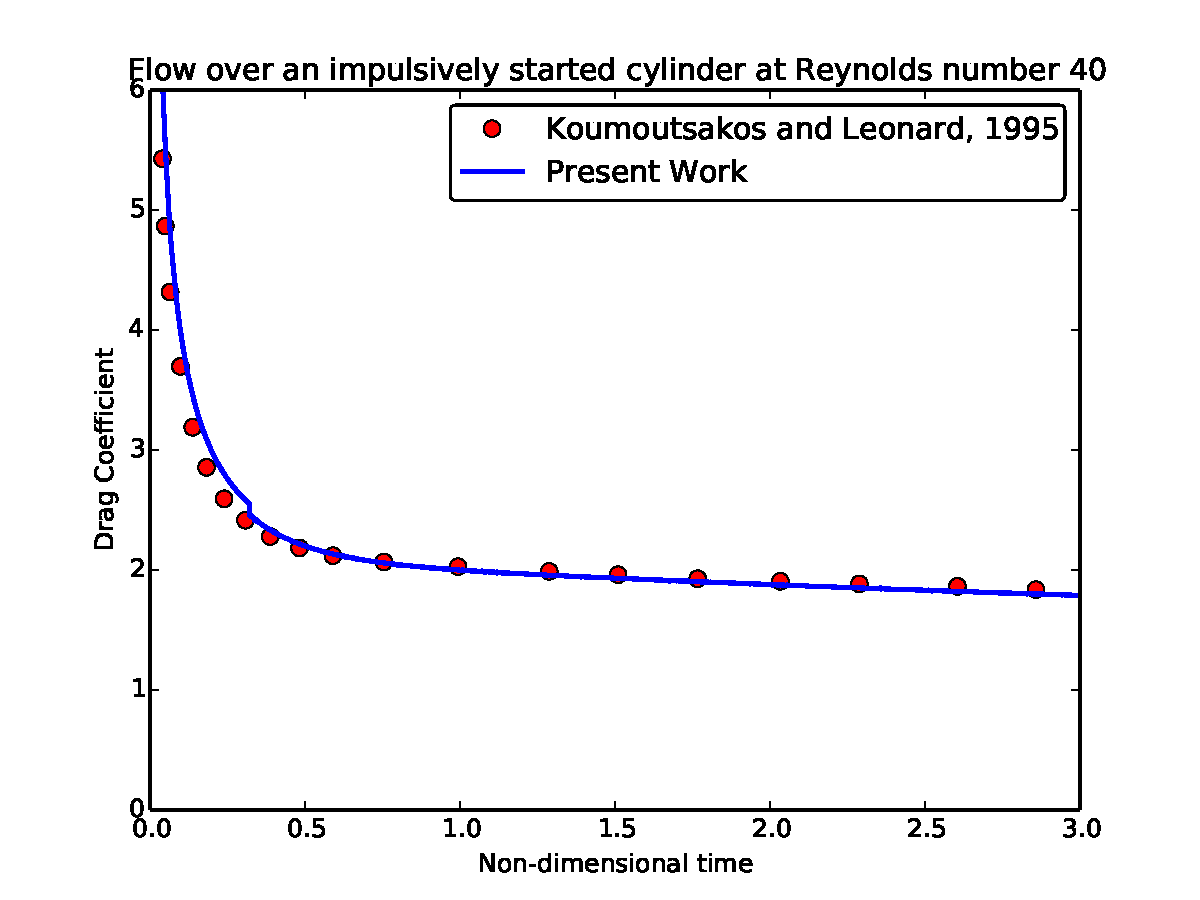
\includegraphics[width=\linewidth]{embedded01}
		\caption{Center spacing h=0.01}
	\end{subfigure}
	~
	\begin{subfigure}{0.4\textwidth}
		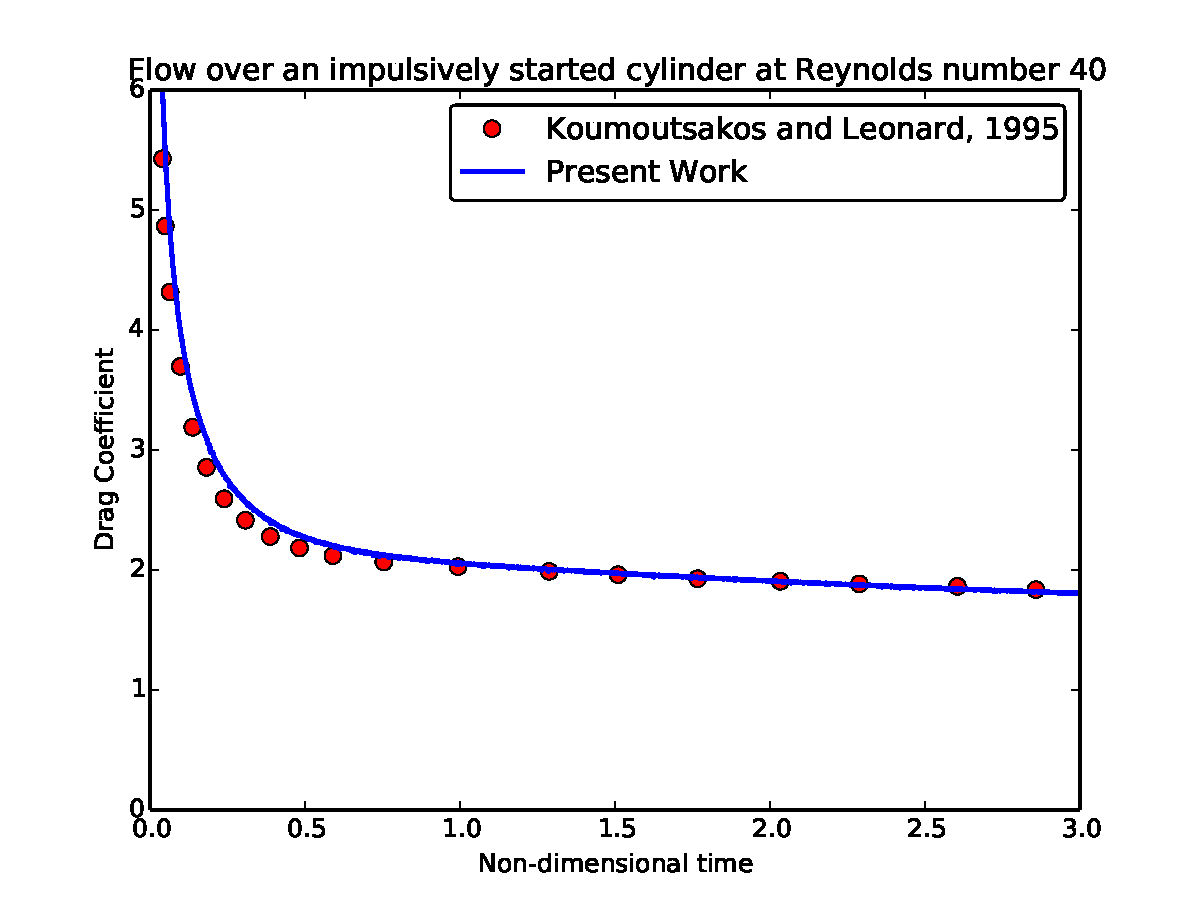
\includegraphics[width=\linewidth]{embedded015625}
		\caption{Center spacing h=0.015625}
	\end{subfigure}
	\caption{Drag force vs time for different grid spacings using the embedded solver.}
	\label{fig:embedded005}
\end{figure}
\begin{figure}[!htb]
	\centering
	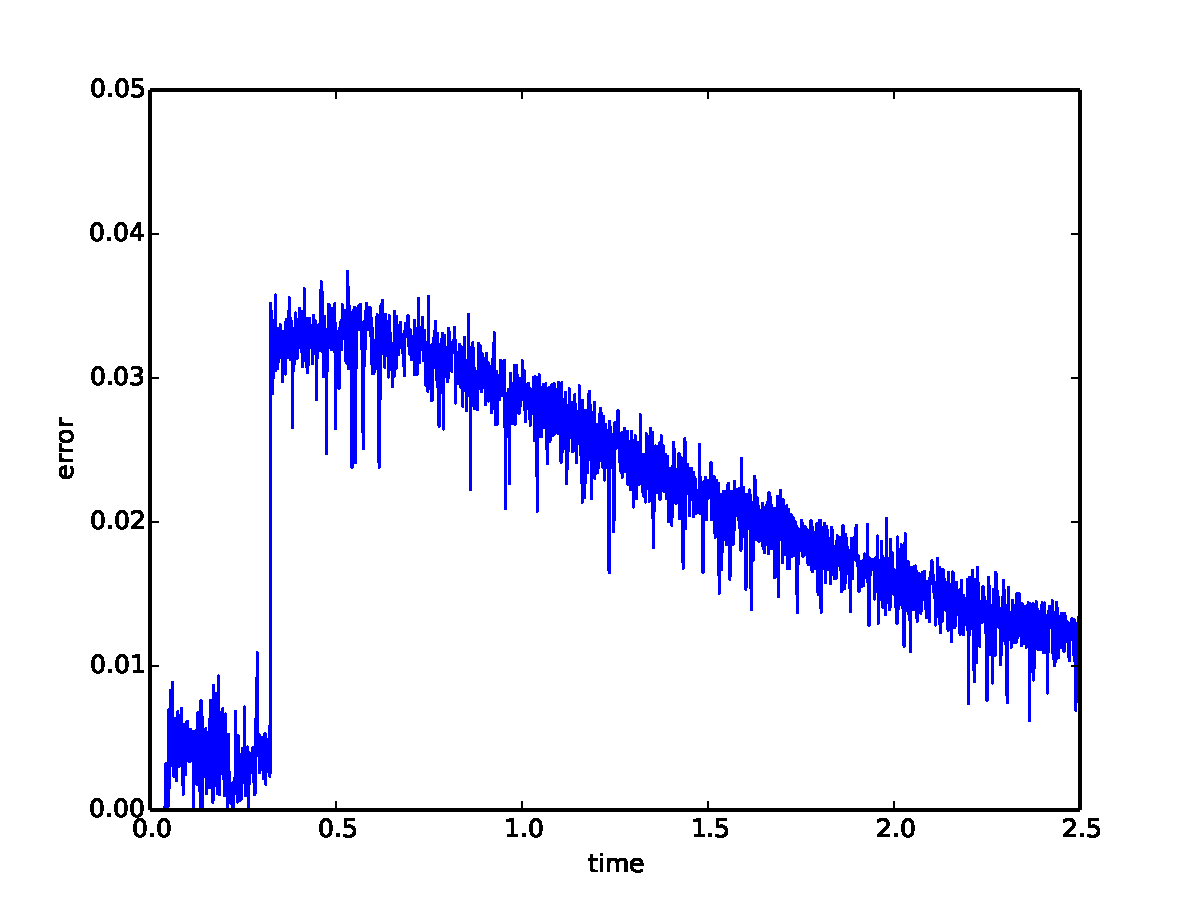
\includegraphics[width=0.4\textwidth]{embedded_error_01}
	\caption{Error in drag force vs time using the embedded method with a center grid spacing of 0.01.}
	\label{fig:embeddederror005}
\end{figure}

Figure~\ref{fig:fadlun005} shows the drag force produced with the modified Fadlun method using grid sizes of 0.005(finest) and 0.025(coarsest).
The finest grid size for the Fadlun method, like the embedded method, also picks up a discontinuity in the force, although at time 0.7.
Unlike the embedded method, the Fadlun method has trouble appropriately handling the jump and ends up creating numerical oscillations. 
The coarsest grid does not pick up the discontinuity and returns a smooth drag curve. 

\begin{figure}[!htb]
	\centering
	\begin{subfigure}{0.4\textwidth}
		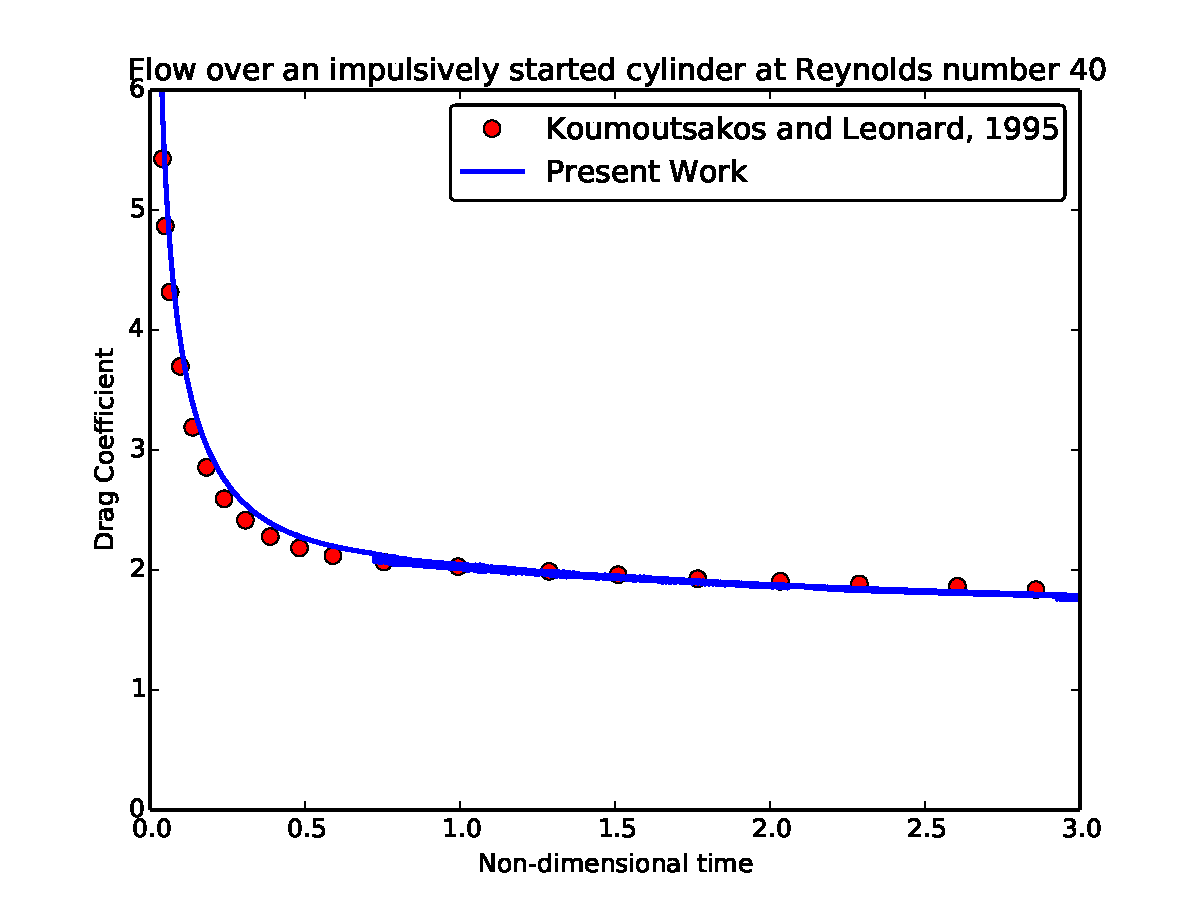
\includegraphics[width=\linewidth]{fadlun005}
		\caption{Fadlun method: grid size 0.005}
	\end{subfigure}
	~
	\begin{subfigure}{0.4\textwidth}
			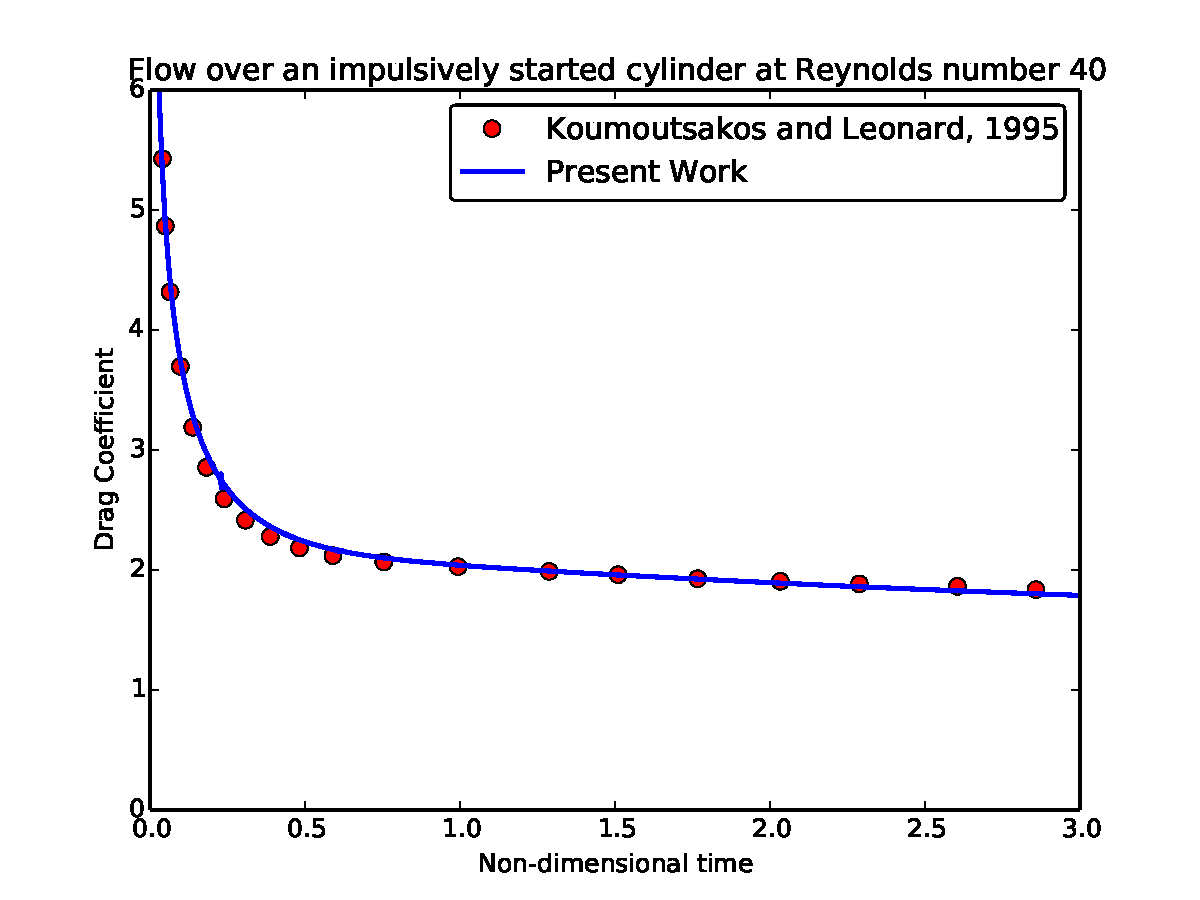
\includegraphics[width=\linewidth]{fadlun03}
			\caption{Fadlun method: grid size 0.03}
	\end{subfigure}
	\caption{Drag force versus time with different grid sizes using the modified Fadlun method.}
	\label{fig:fadlun005}
\end{figure}

A more accurate order of accuracy is presented in Figure~\ref{fig:cyerror2}. 
The order of accuracy here is calculated using the $u$ velocity field. 
Velocity values from the fine grid are bi-linearly interpolated for at the location of velocity values from the coarse grid then turned to error using Equation~\eqref{eq:errorvel}.
\begin{equation}
Error_{avg}=\left(\sum_{nx\cdot ny}^{} \left|\frac{u_{fine}-u_{coarse}}{u_{fine}}\right|\right)/(nx\cdot ny)
\label{eq:errorvel}
\end{equation}
The average error can then be used to calculate the order of accuracy using \eqref{eq:ooa}. 
\begin{equation}
OoA = \frac{\log \left(error_{fine}/error_{coarse}\right)}{\log \left(h_{fine}/h_{coarse}\right)}\label{eq:ooa}
\end{equation}

\begin{figure}[!htb]
	\centering
	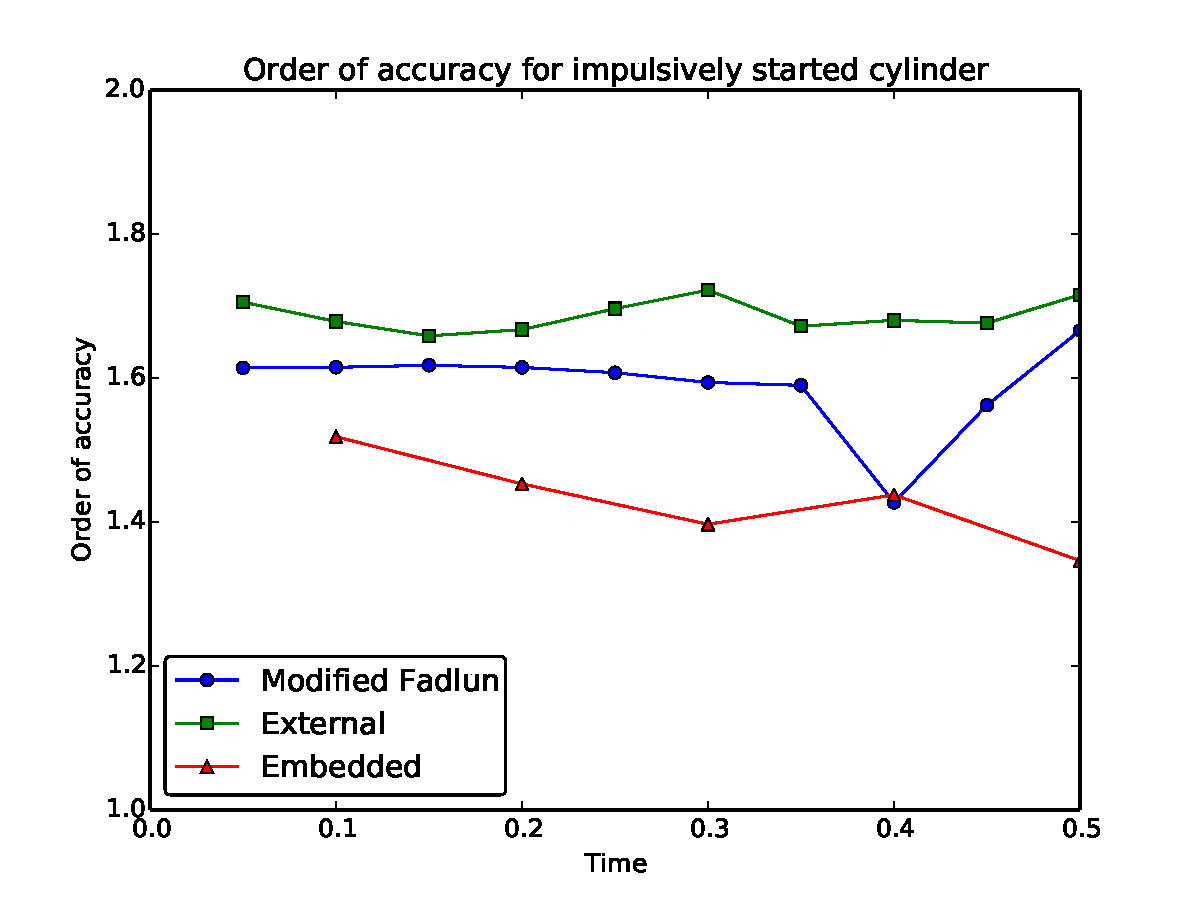
\includegraphics[width=0.4\textwidth]{error_order_2_plt}
	\caption{Order of accuracy calculated at multiple time steps before the discontinuities.}
	\label{fig:cyerror2}
\end{figure}

\subsection{Oscillating cylinder in flow}
The embedded and external methods also have their order of accuracy tested using flow over an in-line oscillating cylinder. 
The modified Fadlun method was not tested here because it proved too unstable to perform with varying grid sizes and time steps. 
Figure~\ref{fig:oscerror} shows the error vs grid spacing plots for the external and embedded methods. 
Interestingly, the two methods have nearly the exact same order of accuracy even though the external method is known to have higher amplitude oscillations as shown in section \ref{sec:osccylinder}. 

\begin{figure}[!htb]
	\centering
	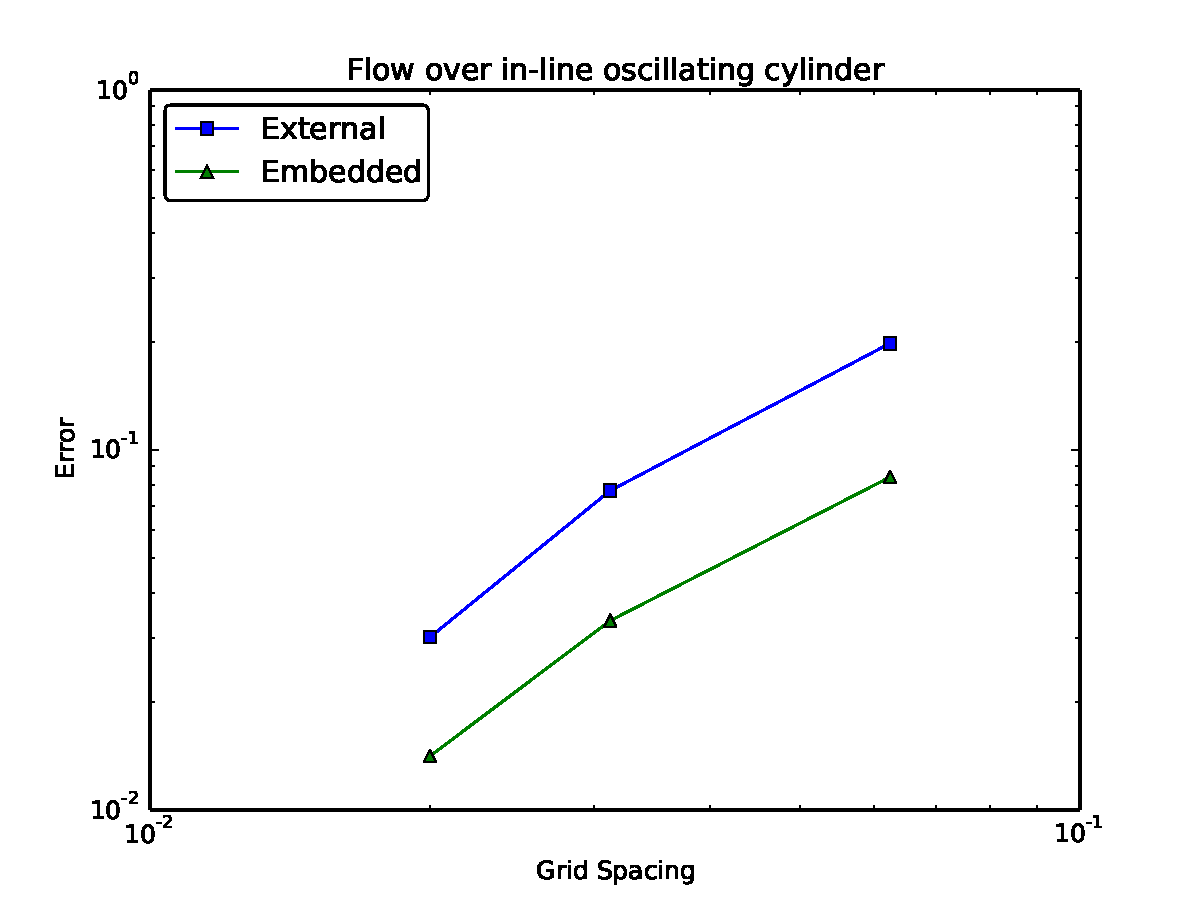
\includegraphics[width=0.4\linewidth]{error_oscflow}
	\caption{Error plotted against grid spacing shows the order of accuracy for the two solvers on the oscillating cylinder in flow simulation.}
	\label{fig:oscerror}
\end{figure}

\section{Performance}
Performance is evaluated by comparing the total number of cells and the computational time. 
Typically, certain parts of the simulation take longer than others. 
The number of iterations taken to solve the Poisson equation give a rough estimate of time taken to solve different parts of the simulation because the Poisson step takes a large majority of the overall time.
Figure~\ref{fig:iter} shows the number of iterations used for each Poisson solve. 
(a), (b) and (c) show the iterations over time for an impulsively started cylinder simulation, and an external and embedded oscillating cylinder in flow simulation, respectively. 
The iteration count is the largest when there is more change in the flow field. 
For instance, in the impulsively started cylinder flow the iterations are  largest at the beginning because the flow fields are going from unity velocity and no pressure gradient to a fully developed boundary layer. 
Note that (a) is solved using the external method which does not have any discontinuities or oscillations in the drag as seen in \ref{fig:embedded005} or \ref{fig:fadlun005}. 
The oscillating cylinder simulation spans two periods with the cylinder starting at $x_{body} =-0.25$ and $u{body} = 0$.
With the embedded method, low Poisson iterations correspond with less numerical iterations which happen when the body velocity is low.
The peaks in the external method seem to happen when the oscillations go from low to high, although the iterations go back down while there is still high numerical oscillation. 
It's worth noting the average iteration count for the external method is around thirty and the embedded method is an order of magnitude more at around 500. 
If the above assertion that iteration count is a rough estimate of time is true then the embedded method should take and order of magnitude more time for the oscillating cylinder simulation.
\begin{figure}[htb]
	\centering
	\begin{subfigure}{0.3\textwidth}
		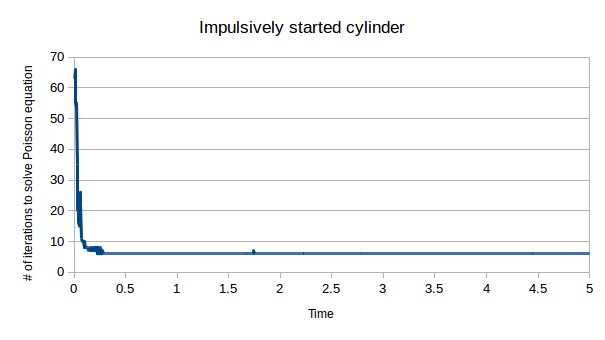
\includegraphics[width=\linewidth]{cy_iter}
		\caption{Impulsively started cylinder}
	\end{subfigure}
	~
	\begin{subfigure}{0.3\textwidth}
		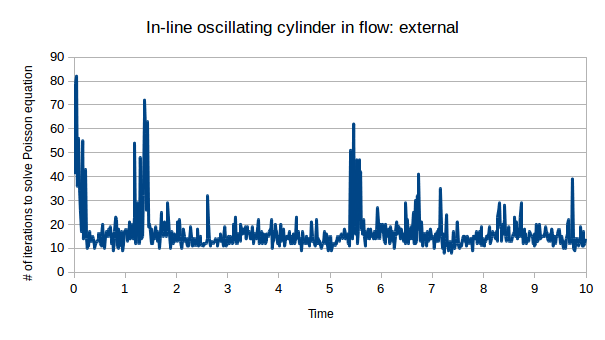
\includegraphics[width=\linewidth]{ex_iter}
		\caption{External oscillating cylinder}
	\end{subfigure}
	~
	\begin{subfigure}{0.3\textwidth}
		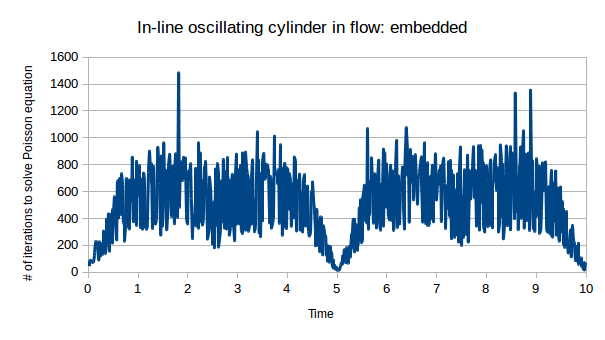
\includegraphics[width=\linewidth]{em_iter}
		\caption{Embedded oscillating cylinder}
	\end{subfigure}
	\caption{Poisson iterations taken to each time step. From left to right: Impulsively started cylinder w/ external method, in-line oscillating cylinder in flow w/ external method, in-line oscillating cylinder in flow w/ embedded method.}
	\label{fig:iter}
\end{figure}

\subsection{Impulsively started cylinder}

Performance of the impulsively started cylinder simulation is evaluated using the same set of simulations as the order of accuracy. 
Figure~\ref{fig:cyperf} shows the performance of all three methods. 
\begin{figure}[!htb]
	\centering
	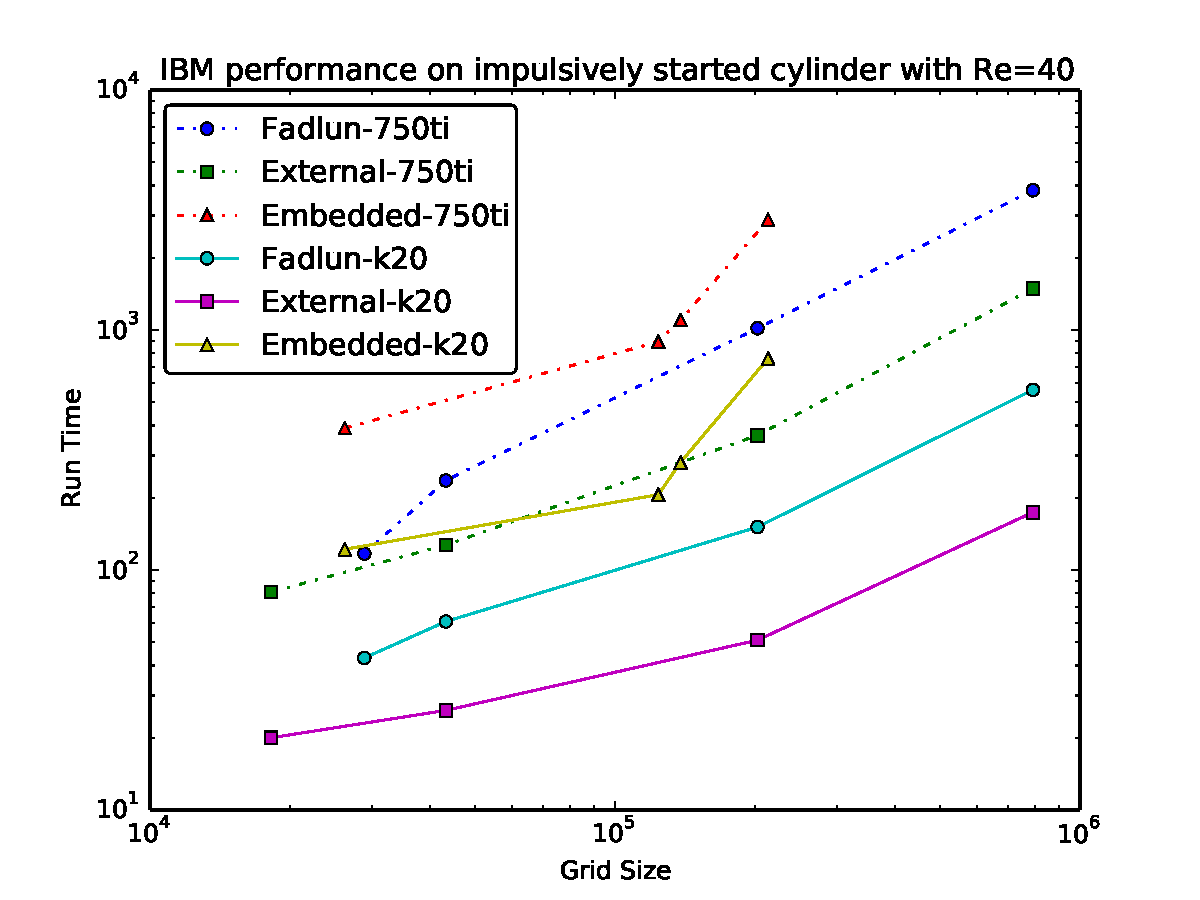
\includegraphics[width=0.4\textwidth]{cylinder_performance}
	\caption{Impulsively started cylinder performance.}
	\label{fig:cyperf}
\end{figure}
It seems counter intuitive that the external method, which is more complex than the Fadlun method performs better. 
This trend surfaces because of the GPU. 
While the external method has complex additional steps, they all end up being trivial to solve on a GPU (from a computational time perspective). 
The time required to perform the interpolations and extrapolations is irrelevant when compared to the Poisson solution. 
Computational time for all three methods, across every type of simulation, is always dominated by the Poisson solver. 
The question then becomes, why does the Poisson solver take longer to solve for different methods? 
Answering this question requires another look at the linear multi-grid method. 
Figure~\ref{fig:gridreduce} shows Poisson stencils on the original grid(left) and a grid reduced by the multi-grid method(right). 
\begin{figure}[!htb]
	\centering
	\begin{subfigure}{0.6\textwidth}
		\includestandalone[width=\linewidth]{grid_reduction}
		\caption{Reduction of the standard Poisson stencil.}
	\end{subfigure}
	
	\begin{subfigure}{0.6\textwidth}
		\includestandalone[width=\linewidth]{grid_reduction2}
		\caption{Reduction of a hybrid node Poisson stencil.}
	\end{subfigure}
	\caption{Grid reduction that takes place inside of the linear multi-grid solver.}
	\label{fig:gridreduce}
\end{figure}
(a) shows the standard stencil that is used for most nodes. 
The modified Fadlun and embedded methods use non-standard stencils near the body because they are both enforcing boundary conditions inside the Poisson solver. 
An example of an atypical stencil, one of the possible stencils for an embedded hybrid node, is shown in (b). 
Linear algebra solvers commonly encounter tri-diagonal, or banded tri-diagonal
matrices that spawn from the discretization of one, two and three dimensional Poisson equations. 
As such, most linear algebra solves are highly optimized algorithms to deal with those types of matrices. 
When non-standard stencils get thrown at the solver, like those found at ghost and hybrid nodes in the embedded method, the solver is unable to efficiently solve the system of equations resulting in more iterations and a longer computational time. 
The external solver is the fastest because it uses the standard Poisson stencil for the entire domain. 

It is worth noting the difference in slope between the three solvers' performance curves. 
If the grid spacing is cut in half the cell count over that domain quadrouples. 
When this happens a non-multi-grid should take approximately four times as long to solve the resulting system of equations.
Theoretically a multi-grid method should be able to achieve better scaling because a lot of the computation is done on reduced grids. 
While the Fadlun and external methods have roughly the same slope, the embedded method is much steeper. 
This implies that the multi-grid method is handling the different abnormal Poisson stencils differently. 
It could be that the clustered, non-standard stencils used at the hybrid and ghost nodes results in the multi-grid solver being unable to sufficiently reduce the grid. 
That could explain the higher order of magnitude of computation time seen with increasing cell count. 

\subsection{Oscillating cylinder}

The performance for the oscillating cylinder is plotted in Figure~\ref{fig:oscperf}. 
Similar trends to the impulsively started cylinder test can be observed here.
Most obvious is the order of magnitude difference in the time taken for each method. 
In addition, the external method scales better with cell count. 
Lastly, it is possible to see another effect caused by GPU scaling which was not visible for the impulsively started cylinder. 
Previously, the more powerful GPU (specifically as measured by the amount of CUDA cores available) achieved roughly the same speedup regardless of cell count. 
Speedup is a term used to measure the difference in speed between algorithms performing the same task e.g. if algorithm \#1 takes ten seconds and algorithm \#2 only takes five then algorithm \#2 achieved a speedup of two. 
For the oscillating cylinder smaller grid sizes have a very low speedup which means that using a more powerful GPU for those simulations is not faster. 
This happens when the non-parallel sections take more time than the parallel sections. 
As cell count increases the parallel portions become larger resulting in a larger speedup. 
\begin{figure}[!htb]
	\centering
	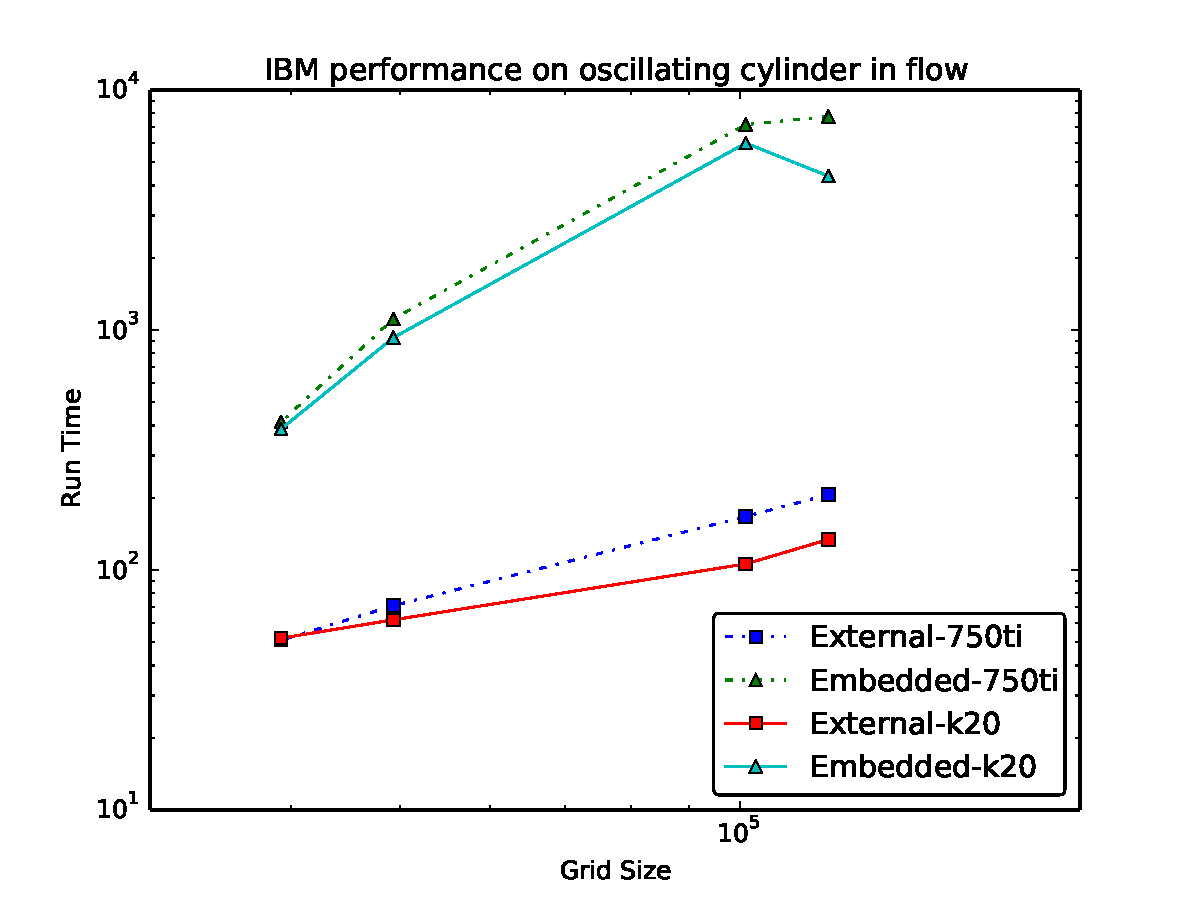
\includegraphics[width=0.4\linewidth]{osc_performance}
	\caption{Performace for flow over an in-line oscillating cylinder.}
	\label{fig:oscperf}
\end{figure}
Figure~\ref{fig:oscperf} is slightly misleading. 
The simulations that comprise it use the same uniform domain size and the same stretching ratios. 
Total cell count is changed solely by changing the grid spacing in the uniform section. 
This graph implies that the overall computational time relies on the total cell count. 
For the most part this implication is true. 
In the previous section it was suggested that the multi-grid solver doesn't properly reduce the grid for the embedded method. 
If this is true than the embedded method should have a negative correlation between grid spacing and computational time(while keeping the overall cell count constant). 
To test this, three grid spacings of 0.0625, 0.05 and 0.03125 were tested. 
The uniform grid section was held constant, ranging from (-1.5,-1.5) to (1.5,1.5). 
The cell count was kept at 224x224 (~60k total) by modifying the stretch ratios. 
Figure~\ref{fig:performance2} shows the resulting computational time. 
Halving the grid size causes the embedded method's computational time to increase by 150\% where the external method only increases by 33\%.
\begin{figure}[!htb]
	\centering
	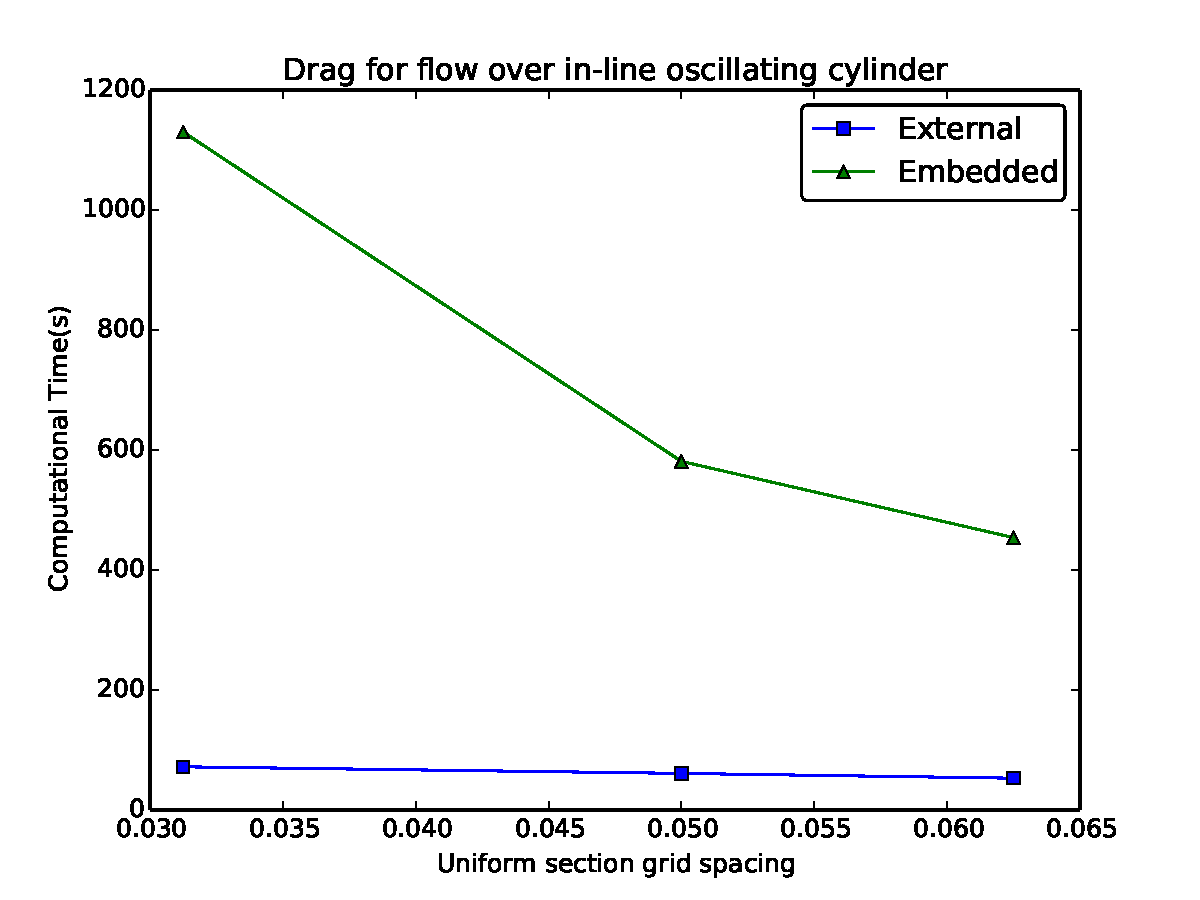
\includegraphics[width=0.4\linewidth]{performance_oscflow2}
	\caption{Computational time for flow over an in-line oscillating cylinder. The total cell count and uniform grid section size are held constant.}
	\label{fig:performance2}
\end{figure}

\chapter{Conclusions} 
Three methods seen here 
overview of each test 
	lid driven cavity 
	impulsively started cylinder 
	osc in no flow + osc in flow 
	VIV 
Which is best for which task
	external for moving bodies.
	plots of VIV forces showing oscillations in external and embedded
	Things that could make the embedded method scale better
		upgrade to amgx?
	potencial multi-gpu scaling
Tie back to original purpose: WEC

\bibliographystyle{plain}
\bibliography{thesis}

\appendix
\chapter{Discretization}
\section{Fadlun}
\subsection{Fadlun Linear Interpolation}\label{Fadlun Linear Interpolation}
\section{Luo}
\subsection{Solving a system of four eqations on the gpu}\label{system of euqations}
\subsection{a: interpolation to hybrid nodes}
\label{a: interpolation to hybrid nodes}

\end{document}
